%%% The main file. It contains definitions of basic parameters and includes all other parts.

%% Settings for single-side (simplex) printing
% Margins: left 40mm, right 25mm, top and bottom 25mm
% (but beware, LaTeX adds 1in implicitly)
%\documentclass[12pt,a4paper]{report}
%\setlength\textwidth{145mm}
%\setlength\textheight{247mm}
%\setlength\oddsidemargin{15mm}
%\setlength\evensidemargin{15mm}
%\setlength\topmargin{0mm}
%\setlength\headsep{0mm}
%\setlength\headheight{0mm}
% \openright makes the following text appear on a right-hand page
%\let\openright=\clearpage

%% Settings for two-sided (duplex) printing
\documentclass[12pt,a4paper,twoside,openright]{report}
% \setlength\textwidth{145mm}
% \setlength\textheight{247mm}
% \setlength\oddsidemargin{14.2mm}
% \setlength\evensidemargin{0mm}
% \setlength\topmargin{0mm}
% \setlength\headsep{0mm}
% \setlength\headheight{0mm}
\let\openright=\cleardoublepage

%% Character encoding: usually latin2, cp1250 or utf8:
\usepackage[utf8]{inputenc}

%% Further useful packages (included in most LaTeX distributions)
\usepackage{amsmath}        % extensions for typesetting of math
\usepackage{amsfonts}       % math fonts
\usepackage{amsthm}         % theorems, definitions, etc.


%\usepackage{bbding}         % various symbols (squares, asterisks, scissors, ...)
%\usepackage{bm}             % boldface symbols (\bm)
\usepackage{graphicx}       % embedding of pictures
%\usepackage{fancyvrb}       % improved verbatim environment
%\usepackage[square]{natbib}         % citation style AUTHOR (YEAR), or AUTHOR [NUMBER]
%\usepackage[nottoc]{tocbibind} % makes sure that bibliography and the lists
			    % of figures/tables are included in the table
			    % of contents
%\usepackage{dcolumn}        % improved alignment of table columns
%\usepackage{booktabs}       % improved horizontal lines in tables
%\usepackage{paralist}       % improved enumerate and itemize
\usepackage{tikz}
\usetikzlibrary{shapes,fit,positioning,snakes,mindmap,trees,decorations.text,arrows.meta}
\usepackage{gnuplot-lua-tikz}
\usepackage{epigraph}
\usepackage{algorithm,algpseudocode}

\usepackage[a-2u]{pdfx}

\usepackage[backend=bibtex8, style=alphabetic, natbib=true]{biblatex} %kvuli podpore citet
\addbibresource{bibliography.bib}

%\usepackage[usenames]{xcolor}  % typesetting in color
\usepackage[textsize=tiny]{todonotes}
\newcommand{\XX}[1]{\textcolor{red}{#1}}

\usepackage{nomencl}
\makenomenclature

%%% Basic information on the thesis

% Thesis title in English (exactly as in the formal assignment)
\def\ThesisTitle{Pattern recognition for in-game spell systems}

% Author of the thesis
\def\ThesisAuthor{Pavel Mikuš}

% Year when the thesis is submitted
\def\YearSubmitted{2018}

% Name of the department or institute, where the work was officially assigned
% (according to the Organizational Structure of MFF UK in English,
% or a full name of a department outside MFF)
\def\Department{Department of Software Engineering}

% Is it a department (katedra), or an institute (ústav)?
\def\DeptType{Department}

% Thesis supervisor: name, surname and titles
\def\Supervisor{Miroslav Kratochvíl, M.Sc.}

% Supervisor's department (again according to Organizational structure of MFF)
\def\SupervisorsDepartment{Department of Software Engineering}

% Study programme and specialization
\def\StudyProgramme{Computer Science}
\def\StudyBranch{Programming and Software systems}

\setlength\epigraphwidth{9cm}
\setlength\epigraphrule{0pt}

% An optional dedication: you can thank whomever you wish (your supervisor,
% consultant, a person who lent the software, etc.)
\def\Dedication{%

\vspace{3 ex}
\noindent
I would like to express my gratitude to Mgr. Miroslav Kratochvíl, the supervisor of this thesis, for his patient guidance, feedback and all the advice he has provided.
I also want to thank my girlfriend for her support and encouragement during the time spent working on this thesis.
}

% Abstract (recommended length around 80-200 words; this is not a copy of your thesis assignment!)
\def\Abstract{%
Magic is a popular element in current computer games. Although most games spoil the sensation of magic as of something extraordinarily subtle by allowing the player to cast spells by simply hitting key combinations, several games require the player to finish a more complicated action before casting a spell: Drawing a complicated glyph that represents the spell is one of such actions. This thesis aims to provide a repurposable library that would allow simple implementation of structured glyph-drawing-based in-game spell systems. The thesis studies several relevant approaches to pattern recognition, describes a neural-network based method for recognition of various shapes and shape combinations, develops a system for describing the parameters and results of the used algorithm in terms of predefined spell shapes and their recognized combinations, and implements this approach in a library and an accompanying simple demonstrational game. The library and its parameters are benchmarked and systematically optimized.
}

% 3 to 5 keywords (recommended), each enclosed in curly braces
\def\Keywords{%
{spell systems} {pattern recognition} {games} {neural networks} {shape combination}
}

%% The hyperref package for clickable links in PDF and also for storing
%% metadata to PDF (including the table of contents).
%\usepackage[pdftex,unicode]{hyperref}   % Must follow all other packages
%\hypersetup{breaklinks=true}
%\hypersetup{pdftitle={\ThesisTitle}}
%\hypersetup{pdfauthor={\ThesisAuthor}}
%\hypersetup{pdfkeywords=\Keywords}
%\hypersetup{urlcolor=blue}

\usepackage{cleveref} %kvuli podpore cref

% Definitions of macros (see description inside)
%%% This file contains definitions of various useful macros and environments %%%
%%% Please add more macros here instead of cluttering other files with them. %%%

%%% Minor tweaks of style

% These macros employ a little dirty trick to convince LaTeX to typeset
% chapter headings sanely, without lots of empty space above them.
% Feel free to ignore.
\makeatletter
\def\@makechapterhead#1{
  {\parindent \z@ \raggedright \normalfont
   \Huge\bfseries \thechapter. #1
   \par\nobreak
   \vskip 20\p@
}}
\def\@makeschapterhead#1{
  {\parindent \z@ \raggedright \normalfont
   \Huge\bfseries #1
   \par\nobreak
   \vskip 20\p@
}}
\makeatother

% This macro defines a chapter, which is not numbered, but is included
% in the table of contents.
\def\chapwithtoc#1{
\chapter*{#1}
\addcontentsline{toc}{chapter}{#1}
}

% Draw black "slugs" whenever a line overflows, so that we can spot it easily.
\overfullrule=1mm

%%% Macros for definitions, theorems, claims, examples, ... (requires amsthm package)

\theoremstyle{plain}
\newtheorem{thm}{Theorem}
\newtheorem{lemma}[thm]{Lemma}
\newtheorem{claim}[thm]{Claim}

\theoremstyle{plain}
\newtheorem{defn}{Definition}

\theoremstyle{remark}
\newtheorem*{cor}{Corollary}
\newtheorem*{rem}{Remark}
\newtheorem*{observation}{Observation}
\newtheorem*{example}{Example}

%%% An environment for proofs

%%% FIXME %%% \newenvironment{proof}{
%%% FIXME %%%   \par\medskip\noindent
%%% FIXME %%%   \textit{Proof}.
%%% FIXME %%% }{
%%% FIXME %%% \newline
%%% FIXME %%% \rightline{$\square$}  % or \SquareCastShadowBottomRight from bbding package
%%% FIXME %%% }

%%% An environment for typesetting of program code and input/output
%%% of programs. (Requires the fancyvrb package -- fancy verbatim.)

%\DefineVerbatimEnvironment{code}{Verbatim}{fontsize=\small, frame=single}

%%% The field of all real and natural numbers
\newcommand{\R}{\mathbb{R}}
\newcommand{\N}{\mathbb{N}}
\newcommand{\F}{\mathbb{F}}
\newcommand{\Z}{\mathbb{Z}}

%%% Transposition of a vector/matrix
\newcommand{\T}[1]{#1^\top}

%%% Various math goodies
\newcommand{\goto}{\rightarrow}
\newcommand{\gotop}{\stackrel{P}{\longrightarrow}}
\newcommand{\maon}[1]{o(n^{#1})}
\newcommand{\abs}[1]{\left|{#1}\right|}
\newcommand{\dint}{\int_0^\tau\!\!\int_0^\tau}
\newcommand{\isqr}[1]{\frac{1}{\sqrt{#1}}}

%%% Various table goodies
\newcommand{\pulrad}[1]{\raisebox{1.5ex}[0pt]{#1}}
\newcommand{\mc}[1]{\multicolumn{1}{c}{#1}}


% Title page and various mandatory informational pages
\begin{document}
%%% Title page of the thesis and other mandatory pages

%%% Title page of the thesis

\pagestyle{empty}
\hypersetup{pageanchor=false}
\begin{center}

\centerline{\mbox{
\includegraphics[width=166mm]{logo-en.pdf}}}

\vspace{-8mm}
\vfill

{\bf\Large BACHELOR THESIS}

\vfill

{\LARGE\ThesisAuthor}

\vspace{15mm}

{\LARGE\bfseries\ThesisTitle}

\vfill

\Department

\vfill

\begin{tabular}{rl}

Supervisor of the bachelor thesis: & \Supervisor \\
\noalign{\vspace{2mm}}
Study programme: & \StudyProgramme \\
\noalign{\vspace{2mm}}
Study branch: & \StudyBranch \\
\end{tabular}

\vfill

% Zde doplňte rok
Prague \YearSubmitted

\end{center}

\newpage

%%% Here should be a bound sheet included -- a signed copy of the "bachelor
%%% thesis assignment". This assignment is NOT a part of the electronic
%%% version of the thesis. DO NOT SCAN.

%%% A page with a solemn declaration to the bachelor thesis

\openright
\hypersetup{pageanchor=true}
\pagestyle{plain}
\pagenumbering{roman}
\vglue 0pt plus 1fill

\noindent
I declare that I carried out this bachelor thesis independently, and only with the cited
sources, literature and other professional sources.

\medskip\noindent
I understand that my work relates to the rights and obligations under the Act No.~121/2000 Sb.,
the Copyright Act, as amended, in particular the fact that the Charles
University has the right to conclude a license agreement on the use of this
work as a school work pursuant to Section 60 subsection 1 of the Copyright Act.

\vspace{10mm}

\hbox{\hbox to 0.5\hsize{%
In .............. date ....................	% FIXME!
\hss}\hbox to 0.5\hsize{%
signature of the author
\hss}}

\vspace{20mm}
\newpage

%%% Mandatory information page of the thesis

\openright

\vbox to 0.5\vsize{
\setlength\parindent{0mm}
\setlength\parskip{5mm}

Title:
\ThesisTitle

Author:
\ThesisAuthor

\DeptType:
\Department

Supervisor:
\Supervisor, \SupervisorsDepartment

Abstract:
\Abstract

Keywords:
\Keywords

\vss}

\newpage

%%% Dedication

\openright

\noindent
\Dedication

\newpage

\openright
\pagestyle{plain}
\pagenumbering{arabic}
\setcounter{page}{1}


%%% A page with automatically generated table of contents of the bachelor thesis

\tableofcontents

%%% Each chapter is kept in a separate file
\todo{predelat na spravny format pdf}
\todo{zeptat se na odkazy u obrazku a odkazy u FANN a URHO3D}
\todo{vytvorit apendix}
\todo{ma byt intorduction chapter s cislem?}

\chapter{Introduction}
Magic has always been a popular part of computer games. In many games, magic has its own lore and laws that make it systematical. Great examples of the complexity of magical spell systems include the games \emph{Magicka} and \emph{Magicka 2}, where the player casts spells by combining eight elements (as seen on \cref{fig:magicka}): For example, using only earth element results in a rock thrown at the enemy, but adding fire will create a classic fireball.

\begin{figure}
  \centering
  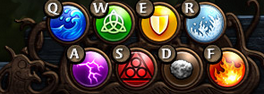
\includegraphics[width=0.5\textwidth]{ext/magicka.png}
  \caption{\emph{Magicka} spell interface}
  \label{fig:magicka}
\end{figure}

In books and movies, wizards can be seen performing complicated hand gestures or drawing complex shapes in order to cast spells. In games, on the other hand, casting magic is usually extremely easy --- the players may often just push a correct button to cause the most advanced magical storms. This spoils the feeling of magic as something extraordinary, complicated, dark, and requiring years of study at the corresponding (imaginary) department of the MFF. Complicated magic systems not only allow the game developers to engage players in a better game experience with the subtle atmospheric feeling of the underlying magic system; the spellcasting itself can also be thought of as a constructive part of the game, requring focus, some amount of creative thinking, and possibly cooperation with other players.

In this thesis, we focus on the constructive kind of spell casting: While the majority of games simply binds spells to buttons, there are several that use some kind of different system. One class of such systems uses pattern recognition algorithms to translate the player's image-like (or, say, rune-like) input to a spell definition. However, as shown in the next section, these systems usually recognize only simple gestures or patterns, which is partly caused by the difficulties in implementing such a system\footnote{In this thesis we ignore other difficulties, which mainly include various marketing and accessibility issues.}. The goal of this thesis is to create a comprehensive pattern recognition system that can be easily plugged into games to allow simple and robust recognition of player-drawn shapes and their translation to an arbitrary spell system.

\section{Pattern recognition in current games}

Symbols and gestures are usually an integral part of the magic, there were many attempts to bring them into video game environment. \citet{gameMagic} provides a following classification of existing gestural systems into three categories (which sometimes overlap or allow an interesting combination):

\todo{Tohle je copypaste nebo rewording? nemuzu najit PDF od ty knizky.}

\begin{description}
\item[Alternative controllers]
Systems may utilize other controllers than mouse and keyboard, such as Wiimote or Kinect. A recent game from this category is \emph{Fable: The Journey}\todo{ref nebo footnote s linkem}, where the player casts spells by moving his hands: For example, push spell is cast by pushing into the air, which is recognized using Kinect technology. While the moves are simple in nature --- they mostly include waving sideways or back and forth --- both hands at the same time can be used, which results in quite complex gestures.

\item[Restricted drawing forms]
A technique used in several games is to let player draw into a predefined grid, or through predefined points. Both \emph{Castlevania: Dawn of Sorrow} and \emph{Deep Labyrinth}\todo{zas linky nebo refy} take advantage of an Nintendo DS drawing interface that allows players to draw magic signs.

In \emph{Castlevania}, players draw signs by connecting glowing points in a circle in out-of-combat situations, as seen in \cref{fig:castlevania}. \emph{Deep Labyrinth} introduces special casting interface that consists of $3\times 3$-grid, where the player connects dots.

The restriction to pre-existing following grid takes away a part of the creative freedom, but makes recognition algorithms much easier to implement and run: For example, only tracing the order of the connected points in \emph{Deep Labyrinth} is sufficient to recognize the spell.

\begin{figure}
\centering
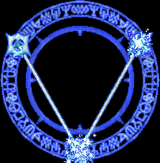
\includegraphics[width=.3\linewidth]{ext/castlevania.png}
\quad
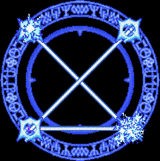
\includegraphics[width=.3\linewidth]{ext/castlevania2.png}
\caption{\emph{Castlevania: Dawn of Sorrow} spell interface \XX{(image taken from ?)}}
\label{fig:castlevania} %label se vaze na caption a musi bejt az po nem
\end{figure}

\item[Free-hand drawing]
One of the first games to integrate some form of pattern recognition of drawn shapes is \emph{Black \& White}. Using a mouse, players (from the role of god) are able to cast miracles by drawing a specific pattern on the ground, as in \cref{fig:blackwhite}. The player can draw anything anywhere on the ground, and its up to the game logic to recognize if the result matches some of the miracle patterns. Alternatively, the player can still cast the miracle by clicking on a button --- presumably because a lot of players had trouble drawing the miracles.

A similar approach to recognition of player-drawn spells is used in \emph{Arx Fatalis}. Players are drawing symbols into the air with a mouse, and a sequence of the drawn symbols represents some spell. While casting, game encodes the mouse moves to letters that represent the 8 directions (with some precision loss). After player finishes the spell, a Levenshtein distance is calculated from each predefined spell sequence to the player's sequence and the one with the lowest Levenshtein cost is returned as a matching spell.

\begin{figure}
\centering
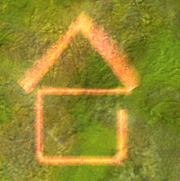
\includegraphics[width=.3\linewidth]{ext/gestureteleport.png}
\quad
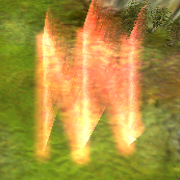
\includegraphics[width=.3\linewidth]{ext/gesturefireball.png}
\caption{\emph{Black \& White} teleport and fireball gestures}
\label{fig:blackwhite}
\end{figure}

\end{description}

\section{Goals}

The result of the thesis allows the players to draw complex spells, preferably more complex than in \emph{Black\&White} or \emph{Arx Fatalis}. For that purpose, we create an algorithm that recognizes a set of basic symbols which can be arbitrarily combined to form new, very complex symbols.

\todo{tadyto asi musis rewordovat, mas to pak nazvany jinak}
Possibilities of such combinations include convolution (symbol is made from other smaller symbols), plain combination (there are multiple symbols next to each other) and embedding (a symbol is put inside another symbol, or into a somehow important position relative to other symbol, e.g. on the top of a triangle). Several examples of symbols and their combinations is shown in \cref{fig:examples}.

\begin{figure}[p]
\centering
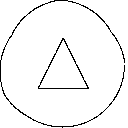
\includegraphics[width=.3\linewidth]{ext/images/embedd.png}
\quad
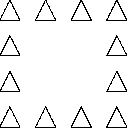
\includegraphics[width=.3\linewidth]{ext/images/comp.png}
\quad
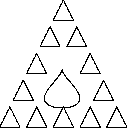
\includegraphics[width=.3\linewidth]{ext/images/comp_and_embed.png}

\vspace{1cm}

\centering
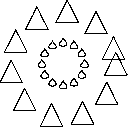
\includegraphics[width=.3\linewidth]{ext/images/comp_in_comp.png}
\quad
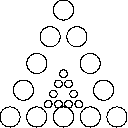
\includegraphics[width=.3\linewidth]{ext/images/comp_in_comp2.png}
\quad
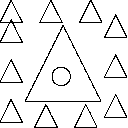
\includegraphics[width=.3\linewidth]{ext/images/triple.png}
\caption{In the figure, embedded positions are always in the middle of the shape. From left to right: circle with embedded triangle; square composed of triangle; triangle composed of triangle, with water drop embedded; circle composed of triangles, with embedded circle composed of water drop; triangle composed of circle, with embedded triangle composed of circle; square composed of triangle, with embedded triangle, with embedded circle in the triangle}
\label{fig:examples} 
\end{figure}


We refrain from using any aiding structures (as e.g. in \emph{Castlevania}) to retain generality of the system.

For the purpose of evaluation the work, we specify the following requirements on the resulting recognition system:
\begin{description}

\item [Durability against shape deformations]
Since we want to recognize hand-drawn shapes, our system has to be prepared for human-like imprecise drawing, especially when drawing with a mouse. However, drawing an exact line between a shape that should still be recognized and a shape that should be rejected is difficult and possibly subjective; we therefore only evaluate the performance on deformed shapes.

\item [Extensibility]
We would like to offer an easy-to-use library that can be used in other projects. For this purpose, the library users need to be able to define their own shapes that should be recognized. The library should act as a framework that offers interfaces for both preparing custom shapes and using them in the pattern recognition process.

\item [Performance]
Our system should be applicable in demanding video games environment, prepared for the possibility of many players drawing their spells at once. To achieve this, we require fast, ideally parallelizable recognition technique.

\item [Recognition of embedded shapes]
To allow players cast complex spells, we need to give them an ability to somehow encode multiple symbols in one spell. One possible way to do it are shape embeddings. Each defined shape can contain several areas, where other shapes might occur. These areas are then processed in our recognition system and classified.

\item [Recognition of shape conglomerations]
For the purpose of this work, we consider shape conglomeration a group of shapes from the same shape class e.g. circle, arranged such that the whole conglomeration forms another shape. We can also look at it as taking the curves of the shape, sampling them uniformly, and then replacing all the samples with the pattern shape.
\end{description}

\subsection{Approach}
The thesis is divided into several steps: First chapter reviews the approaches and algorithms commonly used to solve the pattern recognition problem. We have closely examined three algorithms, namely the \emph{Normalized cross-correlation},\emph{Shape matching and object recognition using shape contexts} and \emph{Matching of Shapes Using Dynamic Programming}. In the same chapter, we describe \emph{Artificial neural networks} and place them in the context of pattern recognition. In \cref{ch:impl}, we describe the implementation of the resulting neural-network-based recognition algorithm. The implementation is accompanied by a simple game prototype that is used to demonstrate the properties of the recognition system. Finally, we perform benchmarking of the performance of our algorithm, with respect to recognition success rate and speed.

In the appendix, we describe the interface of our algorithm and provide a guide for using it in another project. A simple explanation of demonstrational game usage is also included.

\chapter{Pattern recognition}
In this chapter, we describe several classes of algorithms for pattern recognition. In the first part, we review some of the algorithms, namely the \emph{Normalized cross-correlation}, \emph{Shape matching and object recognition using shape contexts} and \emph{Matching of Shapes Using Dynamic Programming}. The second section is devoted to the \emph{Artificial neural networks} in the context of pattern recognition, which are later used for the implementation of thesis goal.

Pattern recognition problem is a broad term for classification problems that are based on the similarity of the features of classified objects. Precise mathematical definition can be found in the work of \citet{formalMethods}. We will focus more on the shape recognition problems category, which is a form of pattern recognition. A shape can be typically defined as an equivalence class under the group of transformations, and the problem is then to algorithmically approximate the human-like visual pattern recognition. \todo{tadyto je furt dost vagni, bud je potreba mit presnou definici tvaru, nebo to vynechat. Ten dalsi odstavec taky. Udelej jednoznacnou definici obrazku (vektorovej nebo bitmapovej s pixlama) a jednoznacnou definici tvaru (neco co v tom clovek z nejakyho duvodu vidi); cimz mas i definici tech tvarovejch trid (mnoziny tvaru ktery clovek oznaci za podobny, nebo existuje nejaka pseudo-metrika ktera aproximuje lidsky rozhodnuti a podle ni jsou taky podobny.}

For example, \citet{simple} propose an algorithm that uses shape context of shape class representant to describe a shape class. The equivalence classes are then defined by a computed distance of the shape contexts of the representant and the shape, and the group of transformations are changes in the shape context.

\section{Algorithms classification}
There are variety of \todo{many?} algorithms on \todo{on je `fyzicky polozeny na', asi ches for?} pattern recognition that can be categorized based on different criteria. \citet{imageRecognition} categorize the algorithms into following approach-based classes:
\begin{description}
\item [Statistical approach] Algorithms in this category are based on the underlaying probability model. The shape class is determined by the features that can be automatically extracted from its members and the probability distributions of the shape belonging to each class. An example of such algorithm is the naive Bayess classifier.

\item [Nonmetric approach] This class contains decision tress, syntactic methods, and rule-based classifiers. The idea of these algorithms is that each shape can be decomposed into the simplest sub-patterns called primitives. These primitives are then viewed as a language and the shape class as a set of rules, from which the shape can be derived. However, the inference of the grammar rules from the training data and the detection of the primitives are difficult problems.

\item [Cognitive approach] Neural networks and support vector machines belong to this class. Neural networks are inspired by biological neural structures. They can be described as massively parallel computation systems that can learn complex input-output relationships.

At the same time, \cite{imageRecognition} remark:
\begin{quotation} However, in spite of the seemingly different underlying principles, most of the neural network models are implicitly similar to statistical pattern recognition methods. \end{quotation}

\end{description}

\cite{skeletonMatching} proposes in the work different classification based on the creation process of the classifier. The algorithms are divided into learning-based approaches and template-based approaches. In the learning-based approaches, pattern classifiers are obtained through training on pre-classified samples. In the template based approaches, patterns are described by templates and the recognition problem is transformed into searching for the best matching template for a given input image.

Another classification proposed by \citet{distanceTransform} divides the algorithms into three classes based on the level of preprocessing:
\begin{itemize}
\item Algorithms that use pixel values directly, e.g. correlation-based methods. Example from this category is the normalized cross-correlation, described in \cref{normalizedCC}.
\item Algorithms that use low-level features such as edges and corners, e.g. distance transform method, described in \citet{distanceTransform}.
\item Algorithms that use high-level features such as identified objects or relation between the features, e.g. graph-theoretic-methods \cite{graph}.
\end{itemize}

Given the amount of algorithms to choose from, we have decided to review only a few of them, namely normalized cross-correlation \todo{cite}, shape contexts object matching and matching of shapes using dynamic programming, and the general approach of using the neural networks, which we use in our algorithm implementation.

\section{Normalized cross-correlation}
\label{normalizedCC}
Following description is based on the work of \cite{crossCorrLewis}.
Cross-correlation is a method to measure the similarity between a template and a given area of an image, both in the form of a grid of pixel values. The term cross-correlation itself means a difference between two signals. It is one of the oldest approaches to pattern and feature recognition and extraction, and still serves as a base for more complex algorithms.

It works by computing the distance between an image and the searched template. We can compute an Euclidean distance of a image f and a template t, where pattern is on a position $(u\,v)$, by comparing corresponding pixels of the image at $(x\,y)$ and the template shifted to $(x-u\,y-v)$.
\[d_{f,t}^{2}(u,v)=\sum_{x,y} [ f(x,y) - t(x-u, y-v) ]^{2}\]
When expanded, it gives us three terms. One of them is the cross correlation term $c(u,v)$.
\begin{align*}
d_{f,t}^{2}(u,v)=&\sum_{x,y} f(x,y)^{2} - 2c(u,v) + \sum_{x,y} t(x-u, y-v)^2 \\
c(u,v)=&\sum_{x,y} f(x,y) * t(x-u, y-v).
\end{align*}

Other two terms express the energy (brightness) of the template and the image, respectively. We perform this computation for all possible values of $u,v$, looking for the lowest value. The we can then consider distances lower than a certain threshold to be a match, and the corresponding $u,v$ terms give us the location.

Computing distance this way has several serious drawbacks. It is computationally demanding since we have to consider every position and every pixel appears in the computation many times, based on the size of the template. The method may also give false matches if the image energy changes a lot with the position. Also, the range of values of cross-correlation term depends on the size of the template and it is not invariant to scaling and rotation.

The performance of the method can be improved substantially if we use convolution. Convolution is an integral that expresses the amount of overlap of one function \emph{g} as it is shifted over another function \emph{f}, which is similar to the cross-correlation. For discrete real valued signals such as pixels of an image, they differ only in a time reversal in one of the signals. We can then apply the convolution theorem.

Convolution theorem \cite{convtheorem} states that when certain conditions are met, Fourier transform of a convolution is an element-wise product of Fourier transforms of input signals. From Convolution theorem follows that time domain or space domain convolution is equivalent to element-wise multiplication in the frequency domain. To compute convolution, we simply need to take element-wise multiplications of Fourier transforms of signals to be convoluted. Cross-correlation differs in that we take the complex conjugate of the Fourier transform of the second signal.

Problems with the range of cross-correlation value and dependency on brightness can be fixed by using normalized cross-correlation, where the image and the template vectors are normalized to unit length. Other desired aspects, such as scale invariance, has been addressed in many algorithms using a cross-correlation method. However, they usually introduce some trade-offs and they may not achieve all the required properties together.

Normalized cross-correlation is defined as:
\[
\gamma(u,v) = \frac{\sum_{x,y}f(x,y) [f(x,y)-\bar{f}_{u,v}][t(x-u,y-v)-\bar{t}]} {\{ \sum_{x,y}f(x,y) [f(x,y)-\bar{f}_{u,v}]^2 \sum_{x,y}[t(x-u,y-v)-\bar{t}]^2\}^{0.5}}
\]
where $\bar{t}$ is the mean of the feature pixel brightnesses and $\bar{f}_{u,v}$ is the mean of the values of $f(x,y)$ in the region under the feature \cite{crossCorrLewis}.

\section{Shape matching and object recognition using shape contexts}
Shape matching approaches that use shape contexts are usually based on the extracted features, which generally introduces a more robust recognition of deformed images. Shape context is usually a group of shape features and their relations and the shape class is then defined by their similarity. We review the algorithm by \citet{simple}. The approach attempts to find corresponding feature points of the image and the template, and then computes their distance as a sum of errors of corresponding points.

We treat an image as a set of points \todo{tohle jsou pixely nebo mnozina bodu co je nekde na tom tvaru?}, and we assume that each shape is represented by a finite subset of its points. We extract from both image and template a certain number of feature points, 100 is recommended by the authors. These points do not need to be the key-points, such as maxima of curvature or corners. This allows us to use a simple extraction method like edge detection.

With feature points extracted, we need to find the corresponding points \todo{in what? in the template? in the tested image?}. To do so, \citet{simple} introduces a \emph{shape context descriptor} \ref{fig:polarbins}, defined by the sample points and their relations. For each sample point $p$, we can create a set of vectors originating from $p$ to all other feature points. Such set of vectors represents positions of other sample points relative to the origin point. The more sample points we choose, the more is this shape descriptor exact.

However, such descriptor might be too detailed and too sensitive to intraclass variations. In the paper, the authors presented a more robust and compact shape descriptor. The idea is that for each point $p$, we compute coarse histogram by assigning other points to bins in polar coordinates with a center in $p$. Polar coordinates are more sensitive to points near p. We can then compute the cost of matching two points as
\[ C_{ij} =  C(p_{i},q_{j}) = \frac{1}{2} \sum_{k=1}^{K} \frac{(h_{i}(k) - h_{j}(k))^2}{h_{i}(k) + h_{j}(k)}, \]

where $ h_{i}(k) $ and $ h_{j}(k) $ represent a $k$-bin normalized histogram at $p_{i}$ and $q_{j}$. Given a set of costs $C_{i,j}$ between all pairs of points $p_{i}$ and $q_{j}$, we need to find the best alignment, which means that we want to minimize the total cost of matching 
\[ H(pi) = \sum_{i} C(p_{i}\,q_{pi(i)}). \]
This can be solved in $O(N^3)$ time using the Hungarian method\cite{simple}. 

\begin{figure}
\centering
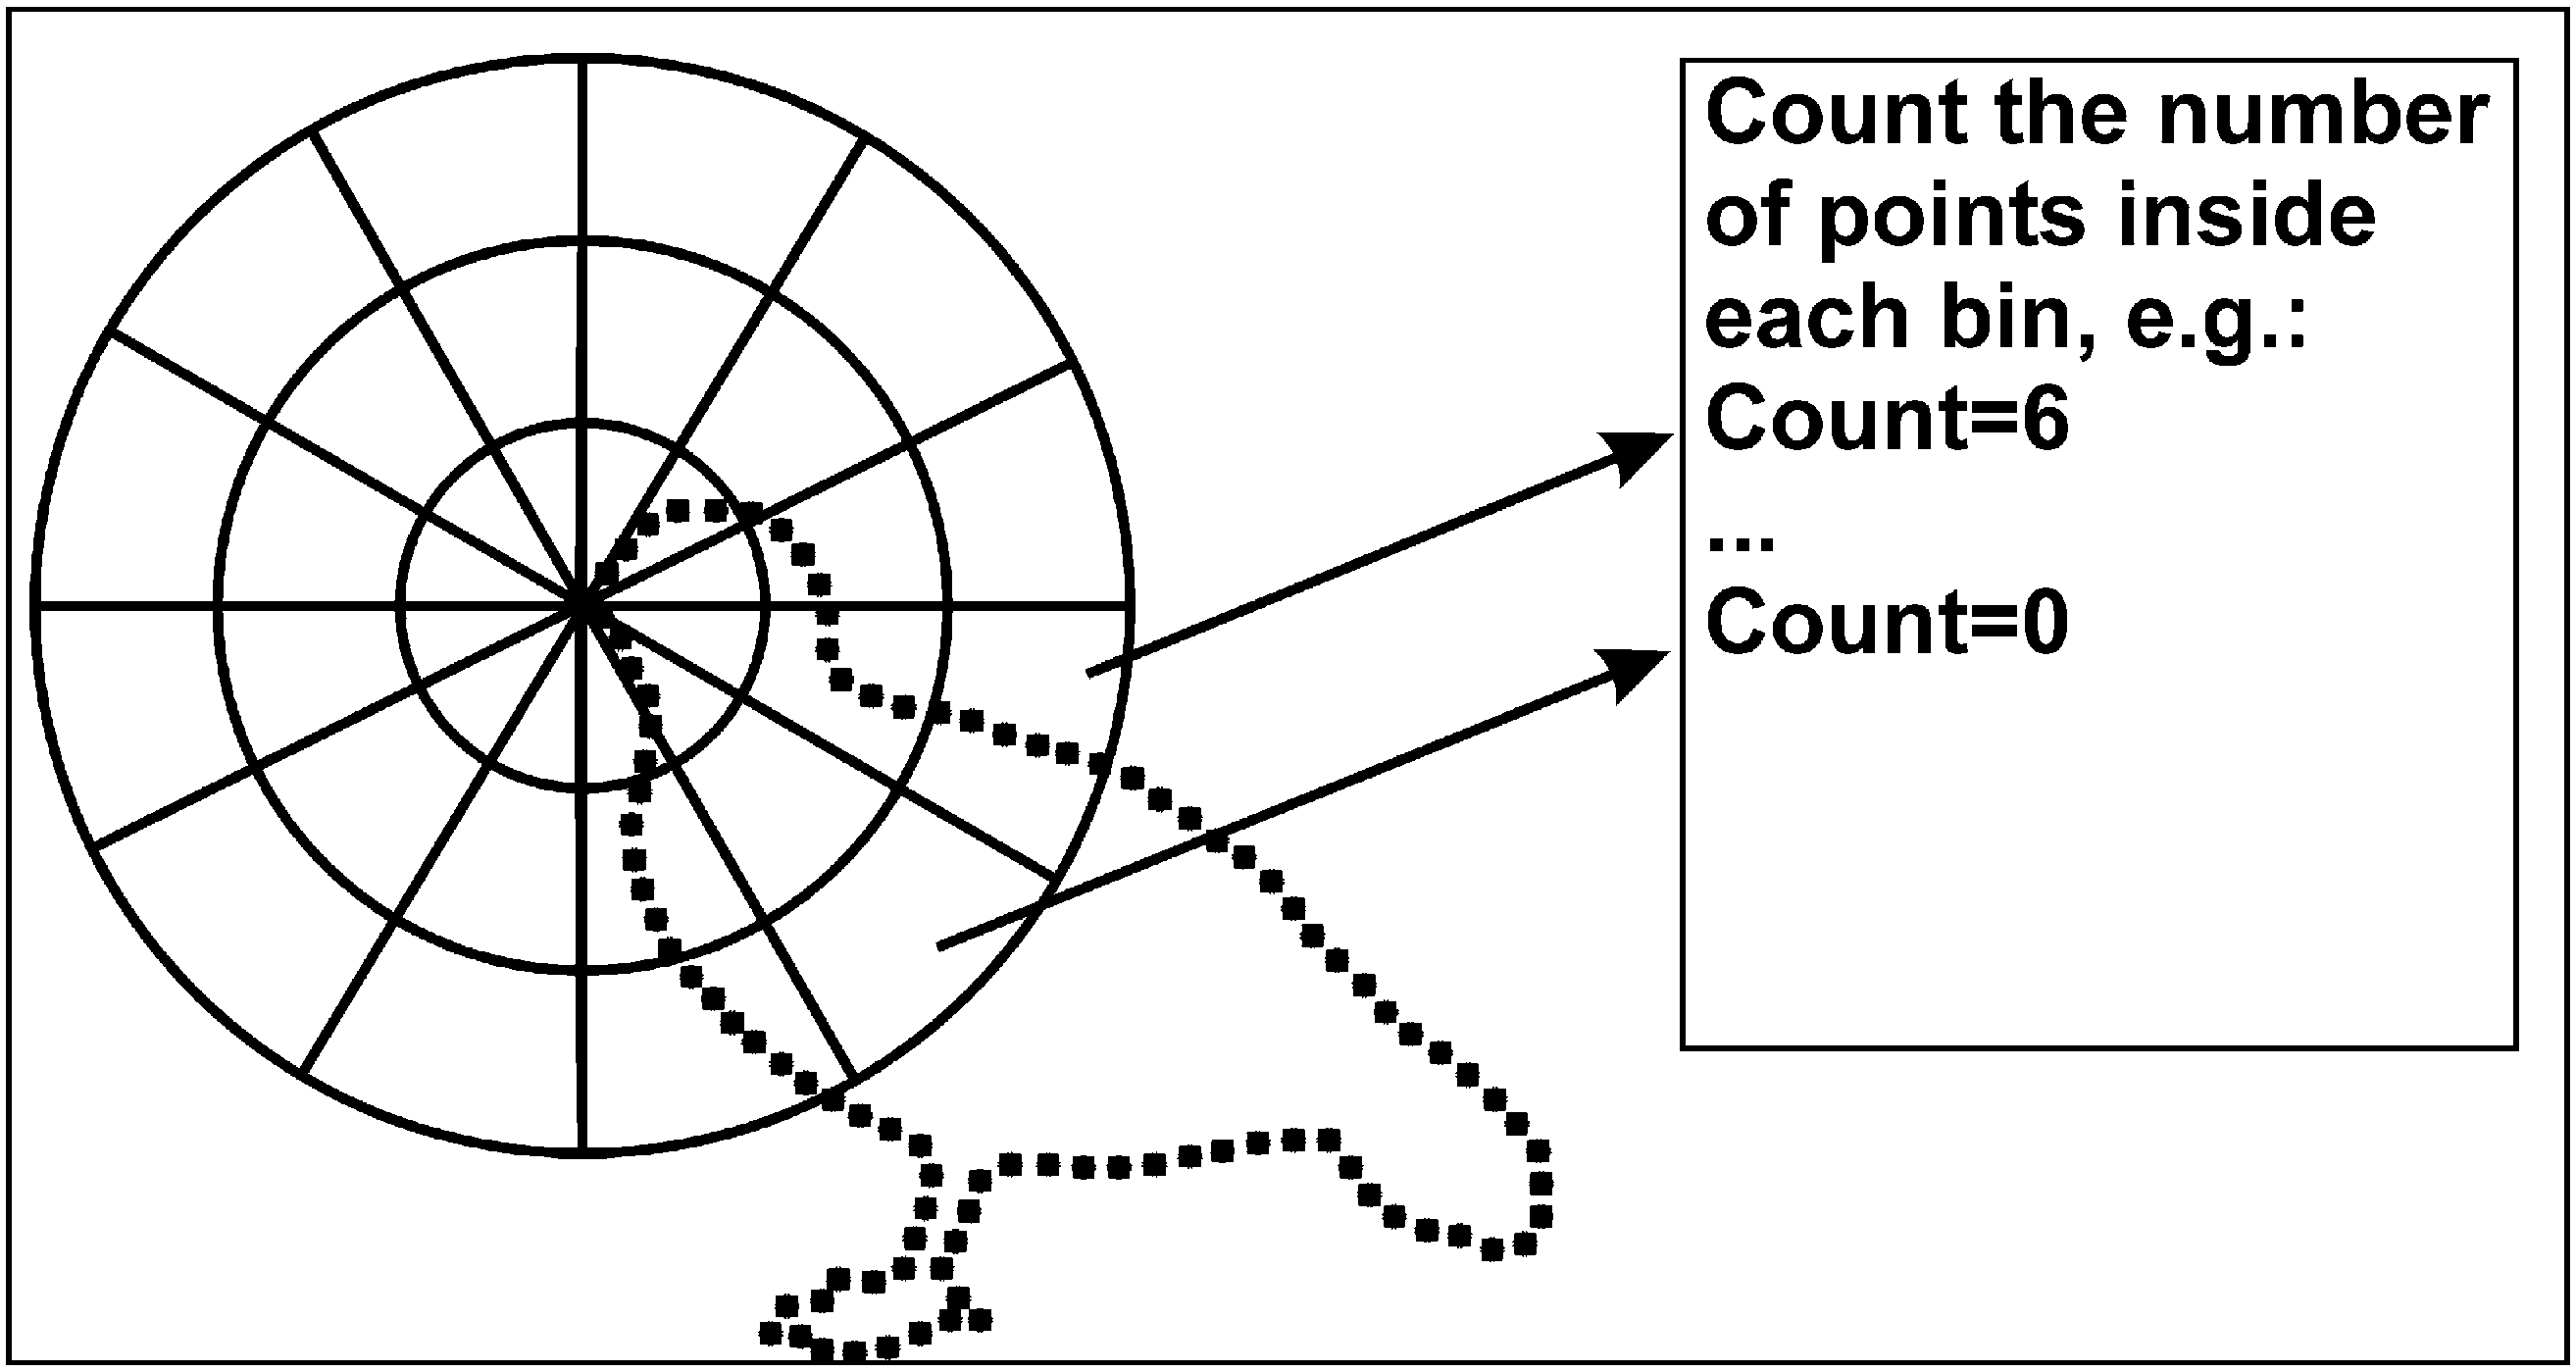
\includegraphics[width=\linewidth]{ext/polarbins.png}
\caption{A scheme of representation of point sets using shape context.
A shape is represented by a discrete set of points sampled regularly along
the contours. For every point, a log-polar histogram—the shape context—is
computed which approximates the distribution of adjacent point locations
relative to the reference point. Image and description taken from \citet{simple}.}
\label{fig:polarbins}
\end{figure}

We can achieve scaling invariance by normalizing all radial distances by the mean distance, and rotation invariance is obtained when searching for the lowest cost among all permutations. According to the paper, this method is also robust against small geometric disturbances.

\section{Matching of shapes using dynamic programming}

A method proposed by \citet{convex} introduces an algorithm which uses dynamic programming combined with high-level features extraction. Similarly to the previous algorithms, the method is based on computation of a distance between the template and the image, but in a different way.

The algorithm requires that the both shape and the template are represented as a sequence of convex and concave line segments, split by inflex points. The idea of the algorithm is to recursively merge segments using two grammar rules $CVC \to C$ and $VCV \to V$, where $V$ denotes concave and $C$ convex segment. Simultaneously, merging cost when the rules are applied is computed using a merging cost function, and the results are stored in the dynamic programming table. The merging cost represents a measure of dissimilarities between the merged segments of the shapes.

Rows and columns of the dynamic programming table represent the inflex points of the shape and the template, respectively. The cost $D(A,B)$ of matching shape $A$ with shape $B$ is defined as:
\[ D(A,B) = min_{T} \{g(i_T,j_T)\}, \]
where $\{g(i_T,j_T)\}$ is a cost of a complete match. The complete match is characterized by a complete path $((i_{0},j_{0}),(i_{1},j_{1}, ..., (i_{T},j_{T}))$, i.e., a path that covers all segments of both shapes. In turn, $\{g(i_T,j_T)\}$ is defined as follows:

\[
g(i_{T},j_{T}) = min_(i_w,j_w) \sum_{w=1}^{T} \phi(a(i_{w-1}|i_{w}), b(j_{w-1}|j_{w}))
\]

Expression $\phi(a(i_{w-1}|i_{w}), b(j_{w-1}|j_{w}))$ represents the dissimilarity cost function defined as: 
\begin{align*}
\phi(a(i_{w-1}|i_{w}), b(j_{w-1}|j_{w}))  = \lambda & \textsc{MergingCost}(a(i_{w-1}|i_{w})) \\
+ \lambda & \textsc{MergingCost}(b(j_{w-1}|j_{w})) \\
+ &\textsc{DissimilarityCost}(a(i_{w-1}|i_{w}), b(j_{w-1}|j_{w}))
\end{align*}

The first two terms in represent the cost of merging segments $a(i_{w-1}|i_{w})$ in shape A and segments $b(j_{w-1}|j_{w})$ in shape B, respectively, while the last term is the cost of associating the merged sequence $a(i_{w-1}|i_{w})$ with the merged sequence $b(j_{w-1}|j_{w})$. Each merging should be a recursive application of the grammar rules  $CVC \to C$ and $VCV \to V$.

The lambda value controls merging tendency. With lower value, merging is more encouraged. For shapes with much detail, it is practical to set higher values, otherwise, these details may be lost during merging. 

At the end of the computation, each field $F(i,j)$ of the dynamic table contains the minimal cost of merging the first $i-1$ segments of the shape and $j-1$ segments of the template. The lower the merging cost is, the more are the segments similar. 

Since the algorithm assumes, that first segments of the shape and the template are aligned and match, we may need to run the algorithm for all possible starting points of shape if we don not know the first segment beforehand.

Differently to the previous algorithm, we now require the extraction of high-level features, we need to extract convex and concave segments in correct order. However, we obtain a matching algorithm that is independent of shape translation, scaling and rotation. We can also directly control the invariance to deformations using the lambda parameter.

\section{Neural networks}
Neural networks are mathematical models of computation inspired by a behavior of a biological nervous system \cite{bishop}. They have been successfully used to solve problems in many different areas, including image and pattern recognition. They can be used to solve problems, where we can not easily mathematically describe the solution given the instance of the problem, for reasons of either complexity or lack of existing mathematical model.

Neural networks have several advantages over the previous methods. They do not require feature extraction since they can learn it themselves, so we can use pixel values directly. They also have a great ability to generalize, which can be used for the recognition of the shape compositions and embeddings. On the other hand, they have to learn to solve the problem before they can be used. 

\subsection{Neuron}
Artificial neural networks are structures based on the parallel computational model of the biological neural systems. The basic network unit is a neuron (see \cref{fig:neuron}), which is characterized by its input and output connection weights, the activation function and a bias. The artificial neural network is built from a number of connected neurons, usually in a layered structure, and the network learning can be characterized as a process of altering the weights of the connections between neurons and the biases of the neurons. 

\begin{figure}
\centering
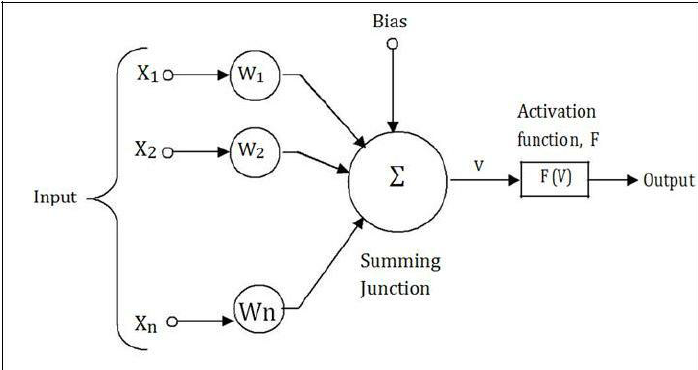
\includegraphics[width=.5\linewidth]{ext/neuron.png}
\label{fig:neuron}
\caption{The model of neuron unit}
\end{figure}

Activation function characterizes the behavior of the neuron. When the values from the input connections are available, the activation function is applied onto the sum of the values and the result is passed further to other neurons. Two common examples of activation functions are the step function and the sigmoid function:

\begin{itemize}
\item $\textsc{Step}(x)=\begin{cases} 1 & (x \geq 0) \\ 0 & (x < 0) \end{cases}$
\item $\textsc{Sigmoid}(x) = \frac{1}{1+e^{-x}} $
\end{itemize}

\subsection{Artificial neural networks}
An artificial neural network is a mathematical model, consisting of a set of neurons interconnected by connections.
More exactly it is a set 
$M  =  (N,C,I,O,w,t)$,  where:
\begin{itemize}
\item $N$  is  a  finite  set  of  neurons.
\item $C \subset N \times N$  is  nonempty  set  of  oriented  connections.
\item $I \subset N$  is  nonempty  set  of  input  neurons.
\item $O \subset N$  is  nonempty  set  of  output  neurons.
\item $w : C \to R$  is  weight  function.
\item $t : N\to R$  bias  function.
\end{itemize}

In practice, multilayer neural networks are commonly used. Multilayer networks are networks, in which the neurons are organized in layers starting with the input layer and ending with the output layer, with hidden layers in between. For each neuron in this structure, its input connections originate only in the previous layer, and its output connections reach only to the following layer.

\subsection{Learning process}
Learning process of an neural network is an optimization problem, where we want to optimize the error function. Error function describes a difference between actual and expected output values for given set of training data. One of the popular error functions is mean square error function:
\[
\textsc{MSE} = \frac{1}{n} \sum_{i=1}^{n} (Y_{i} - \hat{Y}_{i})^2.
\]

Learning process consists of showing inputs to the network and adjusting its connection weights based on the actual and correct output values in order to lower the \textsc{MSE}.

\subsection{Learning algorithms}

\subsubsection{Back-propagation algorithm}
Back-propagation is one of the most popular algorithms for neural networks training, and it serves as a base for many other algorithms.

The algorithm is based on the gradient descent method. In the first step, the input is evaluated and the mean square error of the output is computed. However, a different error function may be used. We can compute the gradient $\frac{\partial E}{\partial w_{ij}}$ for a given training sample using the chain rule
\[
\frac{\partial E}{\partial w_{ij}} = \frac{\partial E}{\partial in_{i}} \frac{\partial in_{i}}{\partial w_{ij}} = 
a_{j}*\frac{\partial E}{\partial in_{i}} = a_{j}*\frac{\partial E}{\partial a_{i}}*\frac{\partial a_{i}}{\partial in_{i}},
\]
where $E$ is the error function, $w_{ij}$ is the weight of the connection between the neurons $i$ and $j$, $in_{i}$ is the weighted sum of the inputs of the neuron $i$ and $a_{i}$ is the output value of the neuron $i$.

If we use the sigmoid activation function denoted $g$, the derivation is:
\begin{equation*}
\frac{dg}{dx}  =  g(x)(1-g(x))
\end{equation*}
which gives us:
\begin{equation*}
\frac{\partial E}{\partial in_{i}} = a_{i}(1-a_{i}) \frac{\partial E}{\partial a_{i}}.
\end{equation*}
We can put the equations together to obtain:
\begin{equation*}
\frac{\partial E}{\partial w_{ij}} = a_{j} a_{i}(1-a_{i}) \frac{\partial E}{\partial a_{i}}
\end{equation*}
There we have two possible cases for the neuron $i$:
\begin{enumerate}
\item [1.] $i$ is an output neuron. Then we get: 
	\[
	\frac{\partial E}{\partial a_{i}} = -(t_{i} - a_{i})
	\]
	where the $t_{i}$ is the expected output for the neuron $i$ for the current input.

\item [2.] $i$ is a hidden neuron. In this case we consider all neurons $k$ that receive input from $i$. Since we are propagating backwards, we know the values $\frac{\partial E}{\partial a_{k}}$ for all $k$. Using chain rule again gives us:
	\[
	\frac{\partial E}{\partial a_{i}} = \sum_{k} \frac{\partial in_{k}}{\partial a_{i}} \frac{\partial E}{\partial in_{k}}
	\]
and from combining the equations we get:
	\[
	\frac{\partial E}{\partial a_{i}} = \sum_{k} w_{ki}a_{k}(1-a_{k}) \frac{\partial E}{\partial a_{k}}
	\]
\end{enumerate}
Now we have defined gradient values $\frac{\partial E}{\partial w_{ij}}$ for all weights in a given neural network.
We can then use the following rule to update the weights:
\[
\Delta^{t} w_{ij} = - \epsilon \frac {\partial E}{\partial w_{ij}} + \alpha \Delta w^{t-1}_{ij}.
\]
$\Delta^{t} w_{ij}$ is the change at time $t$ for the weight $w_{ij}$. The value $\epsilon$ is called the learning rate. If the learning rate is too low, it will take much longer to train the network. If it is too high, the algorithm will cross large section in the search space and will probably oscillate.

In summary, the input is evaluated and the difference between the correct and actual output is computed using error function. The difference is propagated back through the network and weights are updated using the gradient descent method. The whole process is repeated until the desired error value is achieved.

\subsubsection{Quick-prop algorithm}
The quick-prop algorithm is an improved version of the backpropagation. It is based on independent optimization steps for each weight, rather than updating all weights at once. For the update computation, it also requires data from the last iteration, which increases space complexity. The modified $\Delta$ function of the quick-prop algorithm is:
\[
\Delta ^{t} w_{ij} = \Delta^{t-1} w_{ij}*(\frac {\bigtriangledown_{ij} E^{t}} {\bigtriangledown_{ij} E^{t-1} - \bigtriangledown_{ij} E^{t}})
\]
where $\Delta ^{t} w_{ij}$ is the weight delta from $t$-th iteration and $\bigtriangledown_{ij} E^{t}$ denotes partial $w_{ij}$-derivation of error function E in \emph{t} iteration.

\subsection{Advanced structures of neural networks}
There are several advanced techniques in the neural networks field that are commonly used. We describe two of them, the convolution networks and deep neural networks.

\begin{description}
\item [Deep neural networks]
All neural networks with more than two hidden layers can be considered deep neural networks. With the advantage of more layers, deep neural networks can outperform other methods of machine learning. The process of training such network is called \emph{deep learning}. 

More layers allow the network to make more complicated model abstractions over the data. However, there are many challenges to overcome. Deep neural networks have a large number of parameters and training them is demanding on computational power. They are also prone to overfitting, as the added layers of abstraction allow them to find possible unforeseen dependencies in the training data.

\item [Convolutional neural networks]
Convolutional networks can be considered a special case of deep neural networks, because they usually have higher number of layers. They are well suited for pattern recognition directly from the pixels of the image because of their structure of layers with different purposes.
For convolutional networks the convolutional layer is characteristic. This layer is essentially a filter, that performs feature extraction. The filter is composed from neurons that have shared weights, so that the filter performs the same operation on every part of the input. This in turn lowers the number of parameters of the network. Usually, more than one filter is used on the input image, allowing the network to extract different features from the simple ones like edges and corners, to very complex features, such as a house or a tree.
\end{description}

Despite of the performance advantages, we have decided to use the classic feed-forward neural networks with two hidden layers. Because we want to allow the users train the network for their own defined shapes, we need to be able to perform the learning on the user side and offer a simple interface to do so.
This does not correspond well with the advanced neural network structures, which may require certain costly hardware or complicated learning process. Learning of classic neural networks is cheap in comparison, and they can still perform quite well in the recognition tasks.

\subsection{Data preparation for pattern recognition}
Because of their generalization properties, neural network are successfully used in pattern recognition. They are able to approximate an arbitrary mapping between the input values and the output values \cite{bishop}. With this ability, we are not forced to do feature extraction and we can initialize the network with pixel values directly.

It is however recommended to apply several pre-processing transformations that can improve the generalization performance significantly.
\begin{description}
\item [Input normalization]
One of the common forms of pre-processing is input normalization. By applying a linear transformation we can arrange all of the inputs to have zero mean and unit standard deviation over the transformed training set.
In practice, input normalization ensures that the inputs and target outputs stay in unit range, and we can expect that the weights should also be in unit range. We can then initialize the weights with suitable random number. Otherwise, we would have to find a solution, where the weight values differ distinctly.
\item [Training with noise]
Another technique that improves generalization capabilities of the network is training with noise. It involves the addition of a random vector to the input vectors during training. A remark by \citet{bishop} states that:
\begin{quotation} Heuristically, we might expect that the noise will `smear out' each data point and make it difficult for the network to fit individual data points precisely, and hence will reduce over-fitting. In practice, it has been demonstrated that training with noise can indeed lead to improvements in network generalization.
\end{quotation}
\item [Data dimensionality reduction]
Data dimensionality reduction is a pre-processing method that allows the network to have fewer input neurons. It can take the the form of color information removal or pixel averaging, where we group several pixel to one block and use average of each block as an input. By lowering the number of inputs, we lower the number of parameters that the learning process has to optimize.
\item [Feature extraction]
Some of the more complicated techniques use feature extraction as a pre-processing step. Simple geometric primitives extractions are common, such as extraction of lines with their lengths and angles.
\end{description}

\chapter{Implementation}
\label{ch:impl}
In the first part of this chapter we describe the recognition system implemented by this thesis, in the second part we describe the game prototype that demonstrates the usage of the algorithm. Implementation of the recognition system consists of two parts, one responsible for the actual recognition, and one for the training of neural network based on user-defined shapes. The usage of the framework consists of three steps:
\begin{enumerate}
\item Defining the shapes and setting up desired recognition parameters.
\item Training the neural network to classify the defined shapes.
\item Using the framework and the trained network to recognize patterns.
\end{enumerate}

\section{Data representations}
We have developed several data classes that are crucial for the algorithm functionality. The \texttt{ImageLines} is a class that holds the input to the algorithm. The next class is a \texttt{ShapeDescriptor}, an abstract class whose implementations are used to describe shapes, and the last one is a \texttt{ShapeNode} class for the output data representation.

\begin{description}
\item [Image lines class]
We use the vector form in the interface. The shapes are defined as a vector of lines with the start and end point.
The format of input is an instance of the \texttt{ImageLines} class, defined in the \texttt{ImageAnalyzer.h} header file. This class wraps a vector of lines defining the shape, accessible through \texttt{GetImageLines} method. The user is expected to fill the vector with the lines representing the two-dimensional image before passing it into the \texttt{Analyze} method. The class offers several other methods, used primarily by the recognition algorithm. 

A line is represented by the instance of class \texttt{Line}, whose constructor accepts two \texttt{float2} type vectors, first containing the start coordinates of the line, and second containing the end coordinates. Internally, the coordinates are transformed into three-dimensional vectors of a homogeneous coordinate system. 

\item [Shape descriptors]
Shape descriptors are a key part of the system, as they are used both during training of the neural network and during analysis of image. They provide the information about the expected line positions and possible embedded shape locations to the algorithm.

Library user can define their own shapes by inheriting from the abstract class \texttt{ShapeDescriptor} defined in \texttt{ImageAnalyzer.h} file. The shape descriptors use the parametric-like expressions to define shapes. Abstract class functions, which should be defined by the user, take parameter \texttt{t} in the interval $[0,1]$ as an argument, and return a point on the curve in a 2D space in the interval $[0,1]^2$.

The curve does not have to be continuous, but it has to return a value for every parameter value in the range. Thread safety of some methods is also required. It is recommended to keep the shape complexity low, as some very small details may be lost in the data preparation for the training.

\item [Output data format]
Output of the algorithm implementation is in the form of instance of \texttt{ShapeNode} class defined in \texttt{ImageAnalyzer.h} file. It represents a tree structure shown in \cref{fig:output0}, where each node contains the recognized shape index and its pattern shape index. Embedded shapes are contained in a vector of child nodes. Indexes are numbers assigned to each descriptor during algorithm setup, except for the \texttt{unknown} shape index, which serves as a placeholder for unrecognized shapes. We do not differentiate between the empty space and any unrecognized shape.

\begin{figure}[p]
\centering
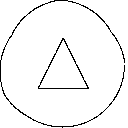
\includegraphics[width=.3\linewidth]{ext/images/example_output0.png}
\quad
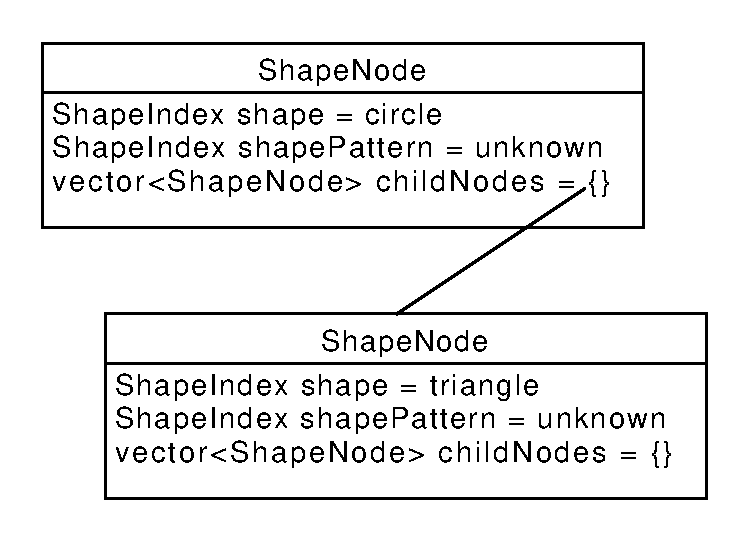
\includegraphics[width=.3\linewidth]{ext/images/example_output0.pdf}
\caption{Input image with expected output. The embeddings form a tree hierarchy, with a single shape in the root and it's embedded shapes as its sons. The \texttt{unknown} shape index marks both unrecognized shapes and empty space.}
\label{fig:output0}
\end{figure}

\begin{figure}[p]
\centering
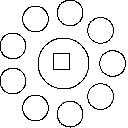
\includegraphics[width=.3\linewidth]{ext/images/example_output1.png}
\quad
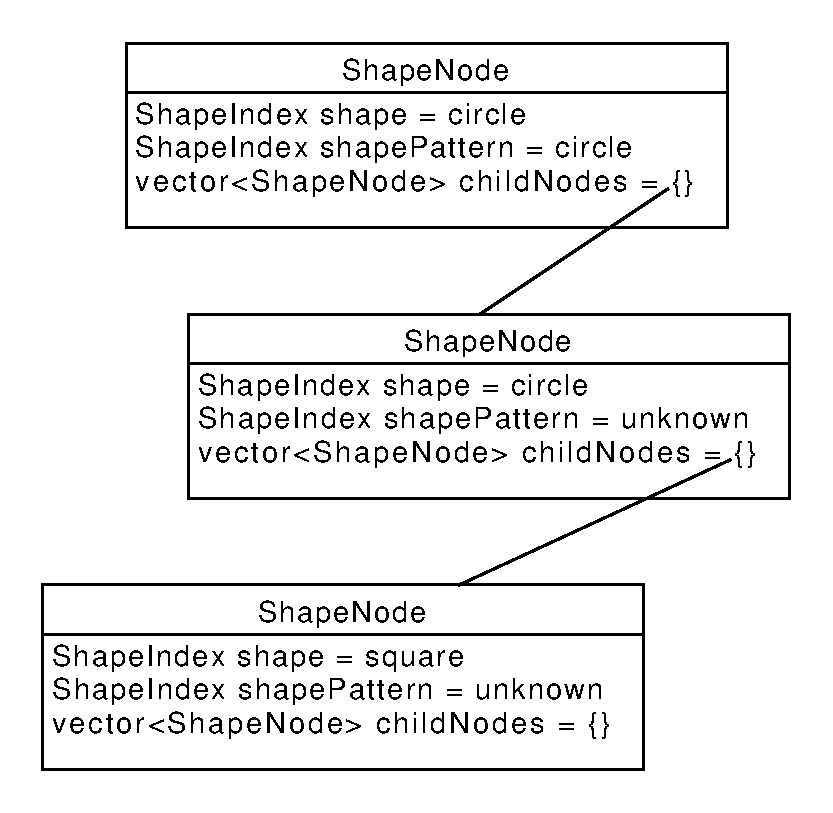
\includegraphics[width=.3\linewidth]{ext/images/example_output1.pdf}
\caption{The output schema for a more complicated image. }
\label{fig:output1}
\end{figure}


\end{description}

\section{Recognition process}
The recognition process is depicted in \cref{fig:algoschema}. It starts in the \texttt{Analyze} method, declared in the \texttt{ImageAnalyzer.h} file. It accepts an instance of \texttt{ImageLines} class as an argument, and returns \texttt{ShapeNode} instance describing the recognized elements in the image.

We have then decided to create the interface for the vector graphics form of input. We expect the input to the program to represent rather simple black and white shapes or their combinations, without any additional information like color or different shades. We also expect the input to be created on the computer in a game, rather than from a photo, and in this environment, it is common to use vector graphics.

\begin{figure}[p]
\centering
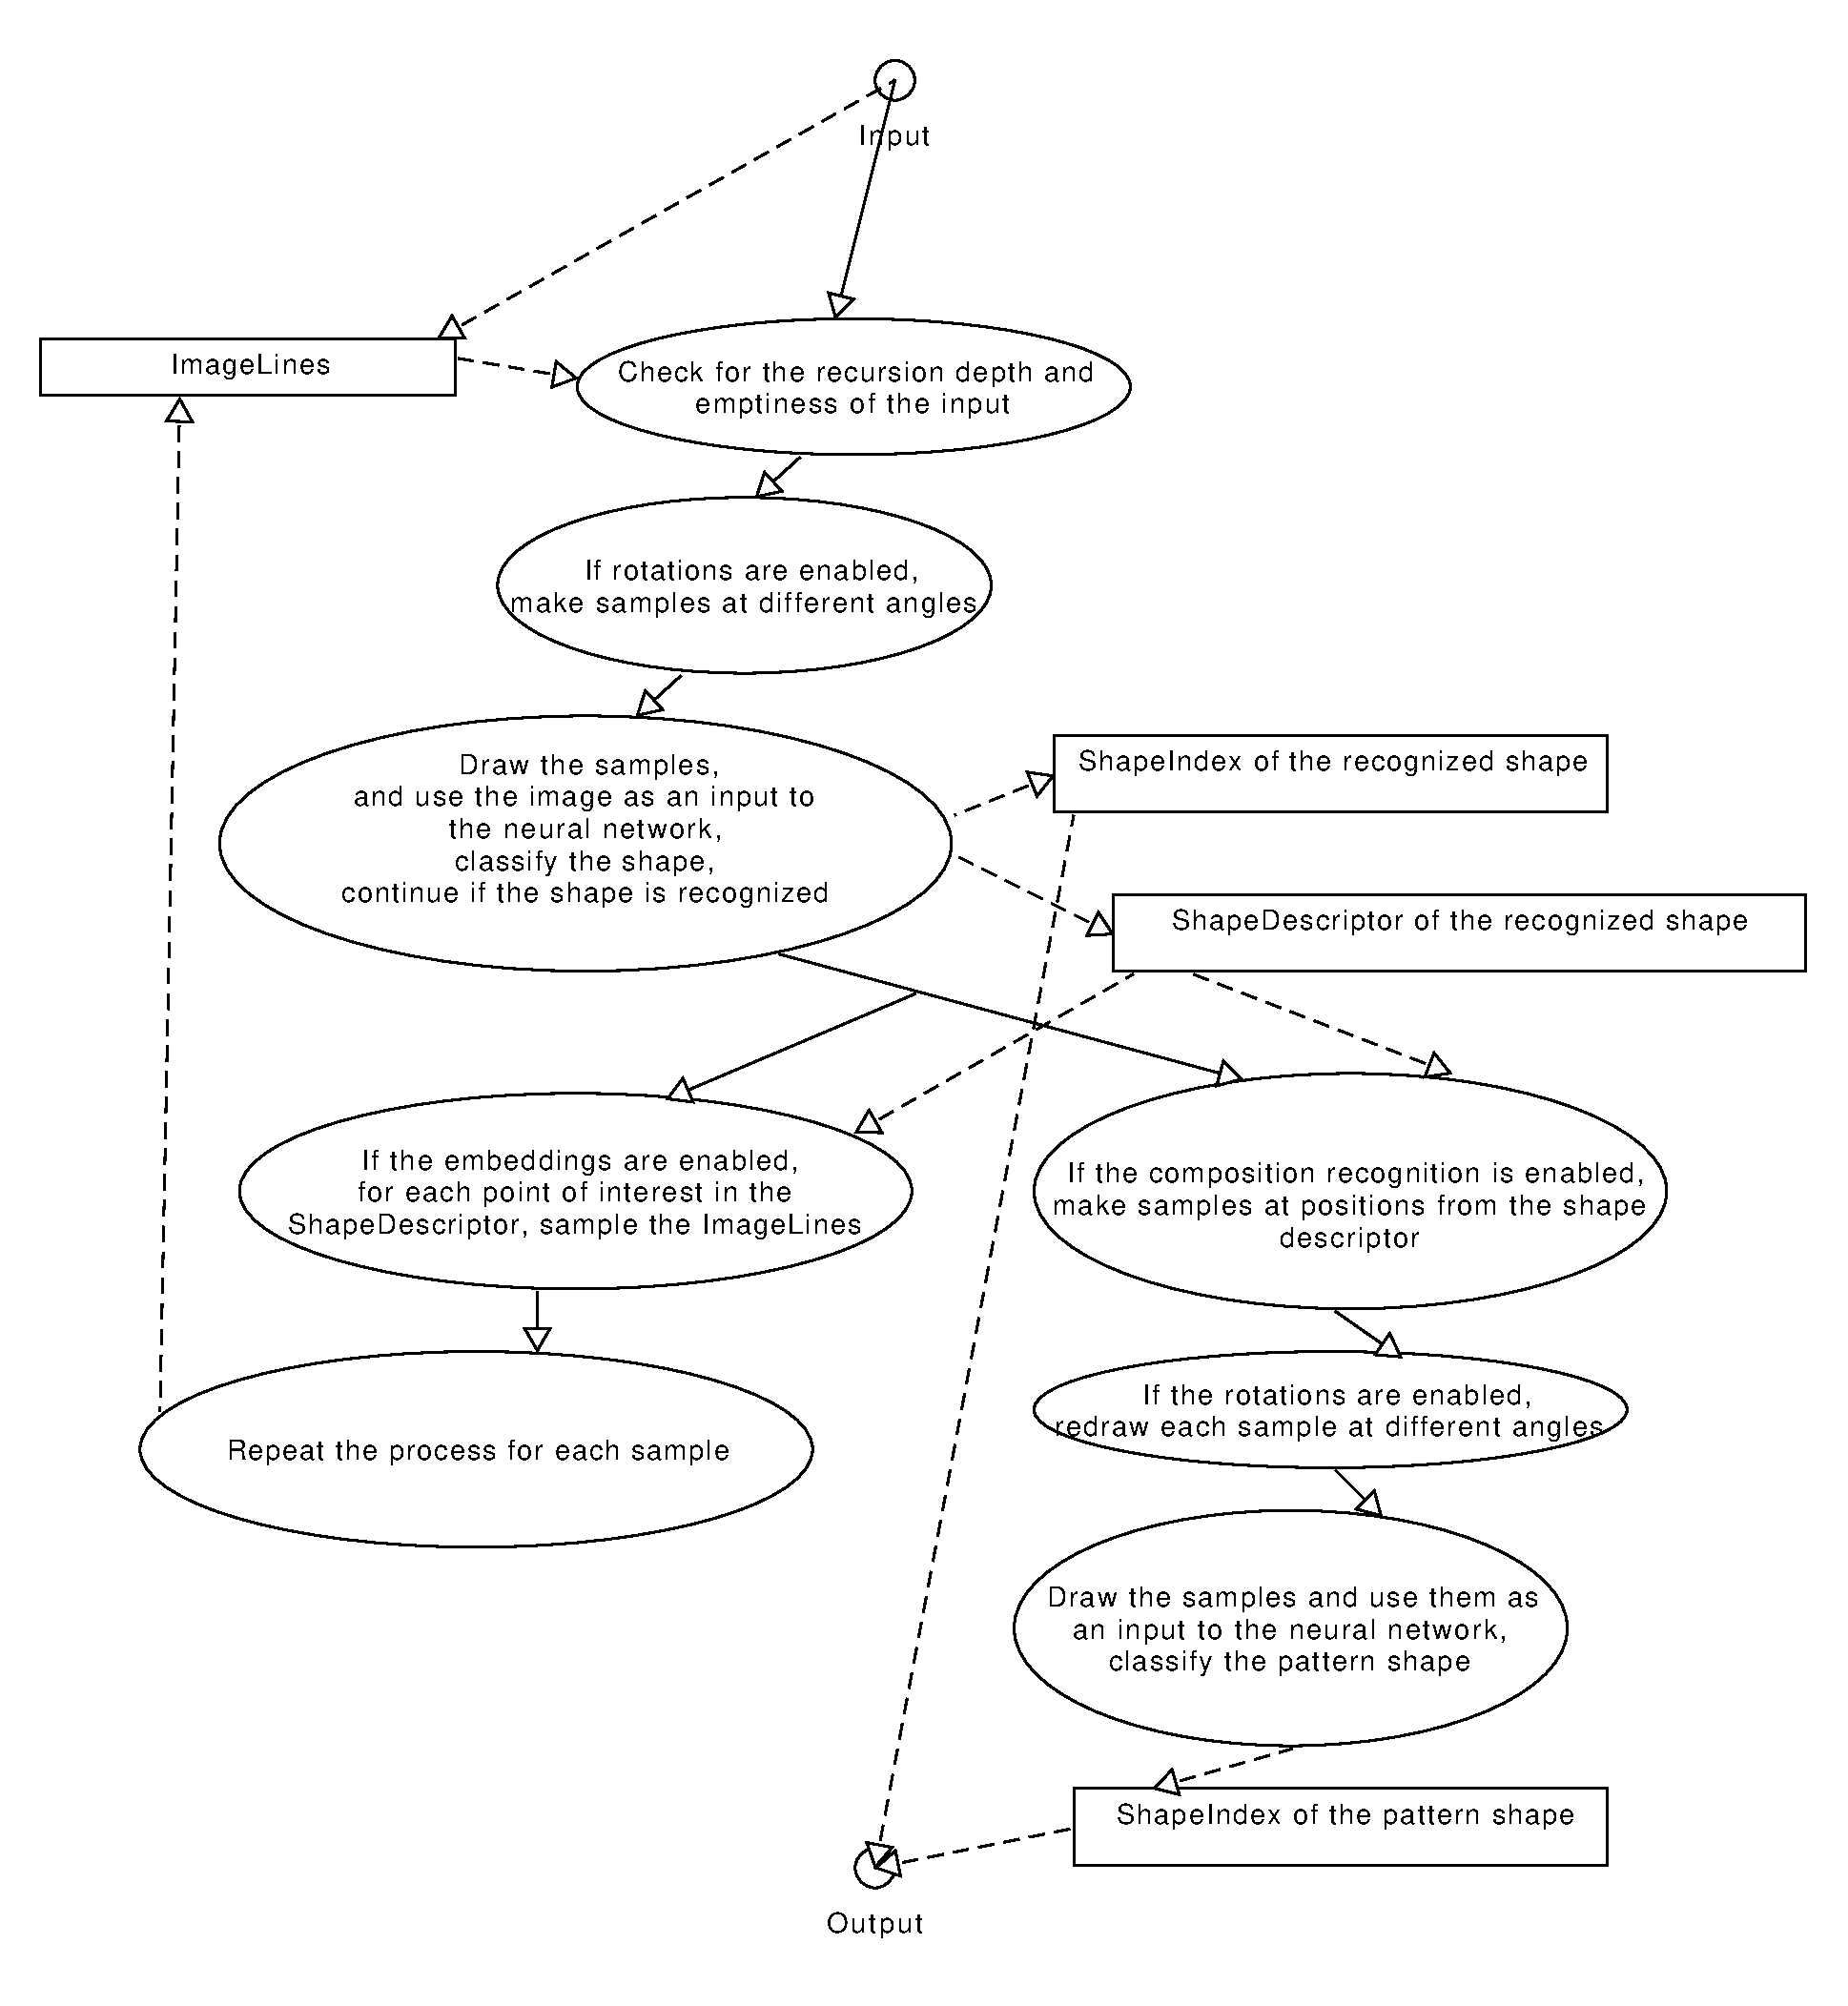
\includegraphics[width=.9\linewidth]{ext/images/algoschema.pdf}
\caption{The figure shows a general algorithm schema. The dashed arrows show appearances of important data structures: \texttt{ImageLines}, \texttt{ShapeIndex} and \texttt{ShapeDescriptor}. The full lines describe the algorithm flow. The algorithm starts with the input, the output is built during the analysis. The algorithm stops when the shape is not recognized.}
\label{fig:algoschema}
\end{figure}

The image lines are first normalized by normalization to the $[0-1]^2$ coordinate space. This transformation is essentially a rescaling, preserving both the length ratios and angles. Then, the top level shape is analyzed by rasterizing the lines into the pixel map which is then passed into the trained neural network.

Generally, the highest neural network output considered to be the matched shape pattern, but only if the value is higher than a user-set constant. There are optionally several more steps involved, described below:

\begin{description}
\item [Rotated shapes] If a recognition of rotated shapes is enabled, the image lines are rotated several times (the exact number is definable by user) by an appropriate angle value, re-drawn and analyzed by the network at each angle.

The network returns a vector of values, each output's value signaling the similarity to the shape assigned to the output, and the highest value is considered the matched shape. If there are several highest network outputs for different rotations with the same value, the first highest value among all outputs is considered. A recognized shape index is returned along with its matching rotation, in which it scored the highest network output.

\item[Composed shape]
When the top level shape is recognized, its shape descriptor is used to sample the theoretical curve points via parameter $t$ uniformly on interval $[0-1]$. If the recognition of rotated shapes is enabled, we transform the sample by an inverse rotation to the matched rotation, to align the recognized shape with the shape descriptor. Then, for each sampled point, this point is expanded into a small square, the original image is clipped to this square, discarding the lines outside, and the result is analyzed. 

Recognized pattern shapes are counted over all samples, and if the count of matches for any shape is high enough, the top level shape is recognized as a composed shape created from a number of smaller shapes of the type with the highest count. Pattern shapes that form the composition are not tested for embedded shapes.

\item [Embedded shape]
To recognize embedded shapes, we use the shape descriptor of the shape recognized previously, and focus on the user-defined embedded shape locations. For each embedded shape location defined in the shape descriptor, we clip the image lines to that area, and recursively run the \texttt{Analyze} method on the result. If the recognition of rotated shapes is enabled, we transform the an area by inverse rotation to the matched rotation, to align the recognized shape with the shape descriptor.
\end{description}

\section{Neural network preparation}
We use the \citet{fann} to train and use neural networks. This open source software is easy to use and install while having a lot of options in terms of network architecture and training. Thanks to its simple interface, we were able to develop an automatized training system for the networks.

\subsection{Training data}
Training the neural network requires a training dataset. Since we want to allow the extensibility in the form of user defined shapes, we have two options. Either to let the user somehow make his own dataset, which is not very convenient, or generate the data procedurally and try to approximate human-like drawing.

We decided for the second option. We generate the data based on the shape descriptors registered by the user and on the algorithm settings. To generate a data sample for the neural network, we take the shape descriptor and create a \texttt{ImageLines} instance from it.

Based on the algorithm settings, it will be either a deformed simple shape instance or an instance of a compound shape. In the case of creating a deformed simple shape, shape curve is sampled many times using the shape descriptor, and the points are connected by lines.
 
To approximate the deformations each point sample can be moved in the direction perpendicular to the line between the original position of the last point, and the original position of the the transformed point. Examples of deformations created by this procedure can be seen in \cref{deformed}.

\begin{figure}
\centering
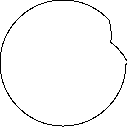
\includegraphics[width=.3\linewidth]{ext/images/deformed0.png}
\quad
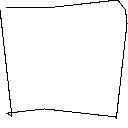
\includegraphics[width=.3\linewidth]{ext/images/deformed1.png}
\quad
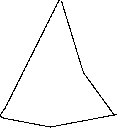
\includegraphics[width=.3\linewidth]{ext/images/deformed2.png}

\caption{Examples of generated deformations of the shapes.}
\label{deformed}
\end{figure}

The transformation  offset is linearly magnified and then reduced, resulting in a heuristics that try to approximate some of the humans like deformations of drawn shapes. Then, the line between the previous and new point is added to the image instance. 

In the case of the shape conglomeration, the shape curve is sampled less frequently and each point is replaced by rescaled image lines of a randomly chosen shape, but this shape is the same for the whole composition. See \cref{fig:examples} for examples.

\subsection{Training}
Training is done using the generated data from the previous methods and the \emph{FANN} library. 
First, the training data and test data are generated,The size of the test data is one-third of the size of training data. Then the network is repeatedly trained on the training data until it reaches the user set up MSE, or until it stops improving.

Internally, the training starts with a high MSE target value, which is then gradually lowered, and in between the improvement ratio is checked. We use the resilient backpropagation (rprop) algorithm from the FANN library, because we achieved best results with this algorithm in terms of the improvements stability. In the neural network, we use an \emph{Elliot} activation function \footnote{The Elliot activation function is:
	$y = \frac {\frac{(x*s)}{2}} {1+\abs{x*s})+ 0.5}$, where $s$ is the steepness parameter.
}.

\section{Game prototype}
The game, which demonstrates the usage of this pattern recognition work, has been developed using the \citet{urho} game engine in version 1.7. Urho3D is, as stated by authors, a free, lightweight, cross-platform 2D and 3D game engine implemented in C++ and released under the MIT license.

\subsection{Game description}
In the game, the player controls the character from a top down view perspective. The player can move and attack the enemies, and, most importantly, cast spells by drawing.

Spells of the game are represented by totem objects --- each time the player casts spell, a totem is created. These totem have different effects on the characters. They can take a form of positive effects that affect the player's character, like healing, or negative effects that affect the enemies, like burning. The task for the player is to survive and destroy all the enemies in the game.

We now describe some of the constructs of the game implementation:

\begin{description}
\item [Drawable texture] \texttt{DrawableTexture} is a component attached to ground in the game. It allows player to draw shapes onto the ground. This component handles the lines sampling and glowing shape line nodes, depicted in \cref{fig:drawing}.

\item [Characters] The player's character and the enemies \ref{fig:start} are represented by a composition of several components: the animated mutant model component, the health component and movement component. The enemies have also an AI component attached, while the player's character has an controller component attached which causes it to listen to the keyboard controls, and the caster component, which allows the character to extract drawn shape from the drawable texture, like in \cref{fig:square}. the caster component also transforms the shape into an \texttt{ImageLines} instance for the recognition.

\item [SpellSystem] The \texttt{SpellSystem} component is a initialization component for the recognition algorithm. It is created only once for the game and the algorithm setup is situated in the constructor. It holds the shape indexes and is responsible for the algorithm output parsing and construction of the spell.

\item [Spell] An instance of a node with the spell component is created each time the player casts a spell. It is a temporary class, serving as a placeholder for the totem object. It invokes the algorithm's \texttt{Analyze} method in a separate thread and waits for the result. This way, the game doesn't freeze while the algorithm analyzes the image. The place of the totem is marked by a green fire, as shown in \cref{fig:orb}, while the image is analyzed. 

\item [Totem] The core of the game are totem objects (see \cref{fig:totem}) and all the spell effects are represented by them. Each totem has a duration for which it exists and an area of effect around it, where the characters are influenced by its presence. The totem can have several effects to it attached. 

\item [Effects]  Effects are components attached to the totems. When a character is inside an area of effect of the totem, the totem applies all of its effects on the character. However, the effects can also be of an single activation type, in which case they are activated only once when the totem is created. An example of such effect is an effect that increases the totem duration.

\item [States] When an effect with duration is applied onto the character, a state component is attached to it, as shown in \cref{fig:effect}. For example, when an over-time healing effect is applied onto a character, the healing state component is attached to the character for a given duration.

\end{description}

\subsection{Spell system}
The game spell system consists of several parts. The first is the \texttt{DrawableTexture} component, which is attached to the ground entity. This component is able to track players drawings and store them as lists of points, each list representing one continuous line.

When the player presses the button to cast the spell, the \texttt{Caster} component attached to their character extracts the lines in a rectangular area around the character and transforms them into the vector of lines. Then the instance of \texttt{Spell} class defined in the \texttt{SpellSystem.h} file is created. There, the \texttt{ImageAnalyzer::Analyze} method is finally called in a different thread and when the analysis is done, the result is parsed and the spell is cast.

\begin{figure}[p]
\centering
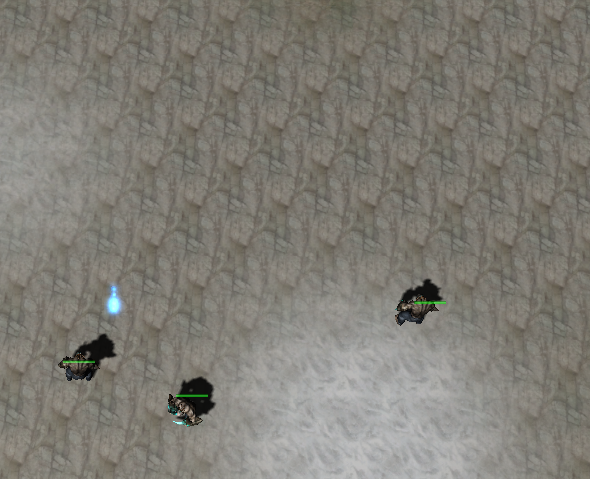
\includegraphics[width=.6\linewidth]{ext/scr/komix1.png}
\caption{There are three mutants in the image, one is controlled by the player, others are controlled by AI. The player starts drawing the spell on the ground by pushing the left mouse button. The mouse position is projected in the \texttt{Caster} component to the game surface and added to the \texttt{DrawableTexture} component which creates a new line.}
\label{fig:start}
\end{figure}

\begin{figure}[p]
\centering
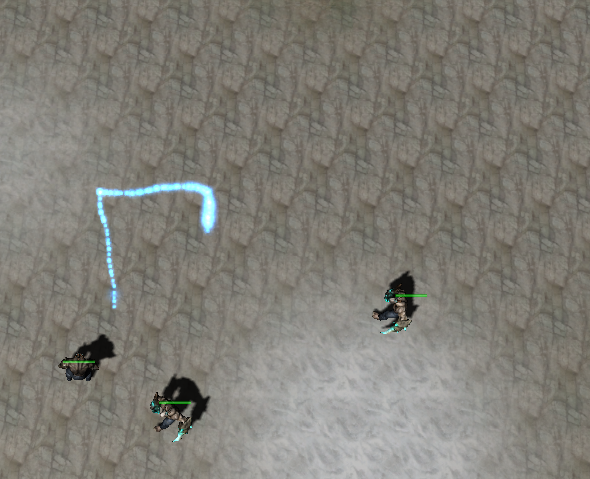
\includegraphics[width=.6\linewidth]{ext/scr/komix2.png}
\caption{The blue glowing line in the image represents the drawing. While the player holds the mouse button, the mouse positions are repeatedly sampled and projected to the surface. The projection points are then added to the line and the space between the points is filled with a blue glow dots to show the line. }
\label{fig:drawing}
\end{figure}

\begin{figure}[p]
\centering
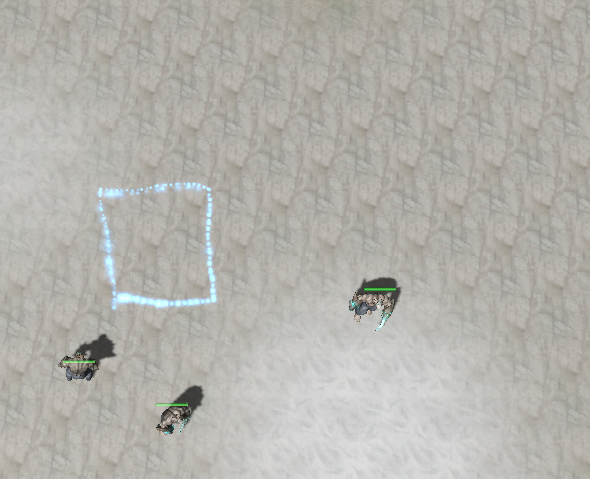
\includegraphics[width=.6\linewidth]{ext/scr/komix3.png}
\caption{The image shows a finished square shape. When the player releases the mouse, the current line is ended. It is possible to continue drawing other shapes. However, when the player casts spell, all lines in a large area around the character are consumed and used for the spell. The extraction of the lines from \texttt{DrawableTexture} and conversion into \texttt{ImageLines} class is done in the \texttt{Caster} component. }
\label{fig:square}
\end{figure}

\begin{figure}[p]
\centering
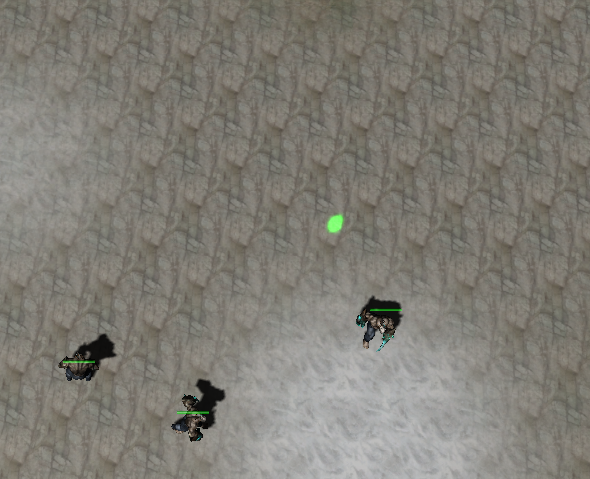
\includegraphics[width=.6\linewidth]{ext/scr/komix4.png}
\caption{When the player casts a spell, the extracted lines are removed and a node with the \texttt{Spell} component is created to handle the spell.  The node is represented by green glowing orb and it marks the place where the totem will be created. It invokes the \texttt{ImageAnalyer::Analyze} method with the lines in another thread to avoid the freezing while the analysis is performed. }
\label{fig:orb}
\end{figure}

\begin{figure}[p]
\centering
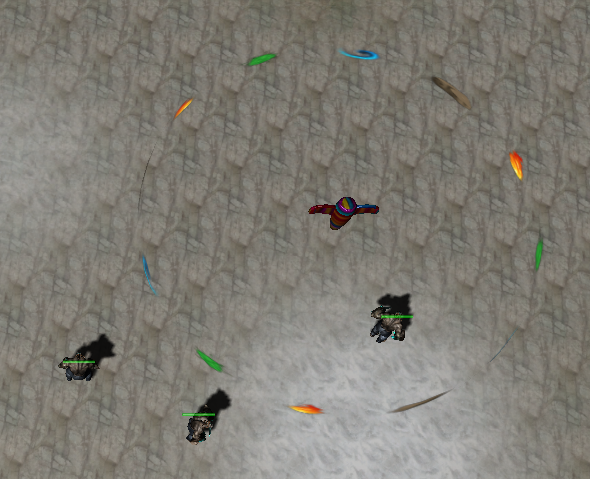
\includegraphics[width=.6\linewidth]{ext/scr/komix5.png}
\caption{When the analysis is finished, the \texttt{SpellSystem} component parses the output. It creates a node with the \texttt{Totem} component, and for each shape, the corresponding effect is added to the totem. The totem is then placed on the spot of the \texttt{Spell}. The totem's area of effect is marked by a rotating circle of elements. }
\label{fig:totem}
\end{figure}

\begin{figure}[p]
\centering
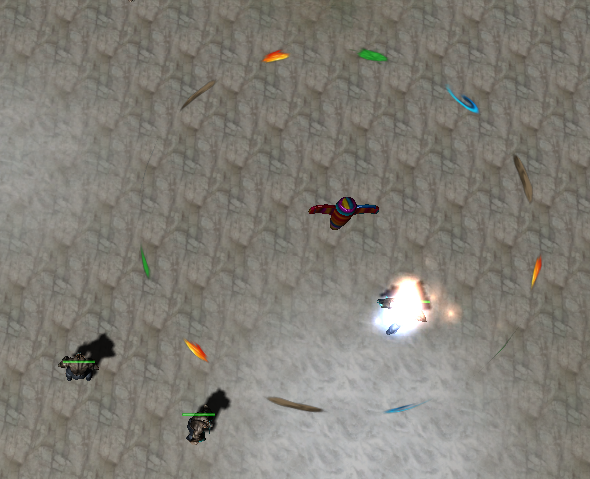
\includegraphics[width=.6\linewidth]{ext/scr/komix6.png}
\caption{The recognized shape was square. Since square represents fire, the totem has the \texttt{FireEffect} component attached to it. When the characters are detected inside the area of effect, the totem applies all of its effect on them. In the figure, the \texttt{FireEffect} is applied to the enemy inside the circle, causing it to have \texttt{FireState} component attached. This component makes the enemy burn, periodically decreasing its health.}
\label{fig:effect}
\end{figure}

\chapter{Results}
In this chapter we evaluate the learning performance of the resulting library. In the first section we describe the process of the optimization of the neural network parameters, in order to achieve the best performance. In the next sections we optimize the parameters of the algorithm and evaluate its performance. For the purposes of evaluation, we have decided to use fixed four shape descriptors, namely the square, circle, triangle and water drop shape descriptors throughout this chapter. If the number of shape descriptors changes, the same method can be applied to re-establish the modified optimal parameters. Examples of the expected inputs of embedding and composition can be seen in \cref{fig:spell:embcircle} and \cref{fig:spell:pattriangle}.
\section{Neural networks performance}
For the correct functionality of the algorithm, it is required that the network is able to recognize the shapes. There are numerous parameters for the neural networks, like the training algorithm choice, architecture and activation function. Because it is not feasible to test every combination of the parameters, we have tested the influence of only a several of these parameters.

\subsection{Setup}
For all the tests we have fixed the following parameters like this:
\begin{description}
\item [Network architecture] All tested networks have a layered structure, with two hidden layers. However, we have tested the influence of different sizes of the layers.
\item [Training algorithm] The networks are trained using resilient back-propagation algorithm from the FANN library.
\item [Activation function] The neurons of the network use the Elliot activation function, a faster version of the sigmoid activation function.
\item [Shape descriptors] We have used four basic shapes descriptors: square, circle, triangle and a water drop throughout the the whole chapter. 
\item [Data] The training data and the test data were generated by the developed generator. The training data consisted of 150 000 images, where each shape had the same amount of examples, and 50 000 images of random data. The test data consisted of 40 000 images of examples of shapes, and 20 000 images of random data. Examples of the data are shown in \cref{fig:trainingExamples}.
\end{description}

\begin{figure}
\vspace{.5cm} %sep
\centering

\includegraphics[width=.1\linewidth]{ext/ex/1.png}

\includegraphics[width=.1\linewidth]{ext/ex/2.png}

\includegraphics[width=.1\linewidth]{ext/ex/3.png}
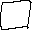
\includegraphics[width=.1\linewidth]{ext/ex/4.png}

\includegraphics[width=.1\linewidth]{ext/ex/5.png}
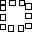
\includegraphics[width=.1\linewidth]{ext/ex/6.png}
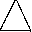
\includegraphics[width=.1\linewidth]{ext/ex/7.png}

\includegraphics[width=.1\linewidth]{ext/ex/8.png}
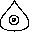
\includegraphics[width=.1\linewidth]{ext/ex/9.png}
\caption{9 examples of auto-generated training data. The resolution of each image is 32*32 pixels.}
\label{fig:trainingExamples}
\vspace{.5cm} %sep
\end{figure}

\subsection{Tested parameters}
We have tested the combinations o the following parameters:
\begin{description}
\item [Layer size] We have tried several values for both layers. For the first hidden layer, we have tried 100, 200 and 300 neurons, and for the second hidden layer 10, 20 and 30 neurons. These values were chosen heuristically from the range recommended by \citet{layerSize}.
\item [The value of MSE] We have trained the networks at different levels of precision, with the target MSE values of 0.1, 0.07, 0.04 and 0.01.
\item [Algorithm settings] The neural networks were trained for different combinations of algorithm settings, with embeddings and composition turned off and on.
\end{description}
We trained the networks with all the combinations of the parameters above, which gave us a total of 150 trained neural networks to evaluate.

\subsection{Evaluation}
The networks were evaluated in the following scenario. For each of the combinations of embeddings and composition being turned on or off, the dataset of 1000 images was generated, with the same amount of examples for each shape. Then, the network was assigned a score computed as a sum of scores over all examples. Score per example was assigned by the following rules, in order to mimic the actual usage in the algorithm, where we consider only the maximum output:

\begin{description}
\item [1] If the maximum of the outputs of the network is in the corresponding output neuron of the shape that is in the example, which means, that the network classified the shape correctly.
\item [2] If the maximum of in the correct output neuron and is higher than 0.7. 
\item [-1] If the maximum is in the wrong output neuron which corresponds to the different shape than the one in the image, and the value is higher than 0.7.
\item [0] Otherwise.
\end{description}

These rules \label{rules} mimic the usage of the network in the algorithm, where only maximum values above 0.7 are considered. The value 0.7 was chosen because the scores of the networks differ more with a numbers closer to 1, and the plots are more clear. From the rules it follows that each network could achieve a score in range from -1000 to 2000 on the dataset of 1000 samples.

\subsection{Results}
\Cref{fig:simples,fig:embed,fig:comp,fig:cmb} show the score of the networks achieved on different evaluation datasets. The datasets contain 1000 samples each, but differ in the techniques used in the images. The first dataset contains only simple shapes, without embeddings or conglomeration, the second contains embeddings only, the third composition only, and finally the fourth contains both embeddings and composition combined.

\begin{figure}
\centering
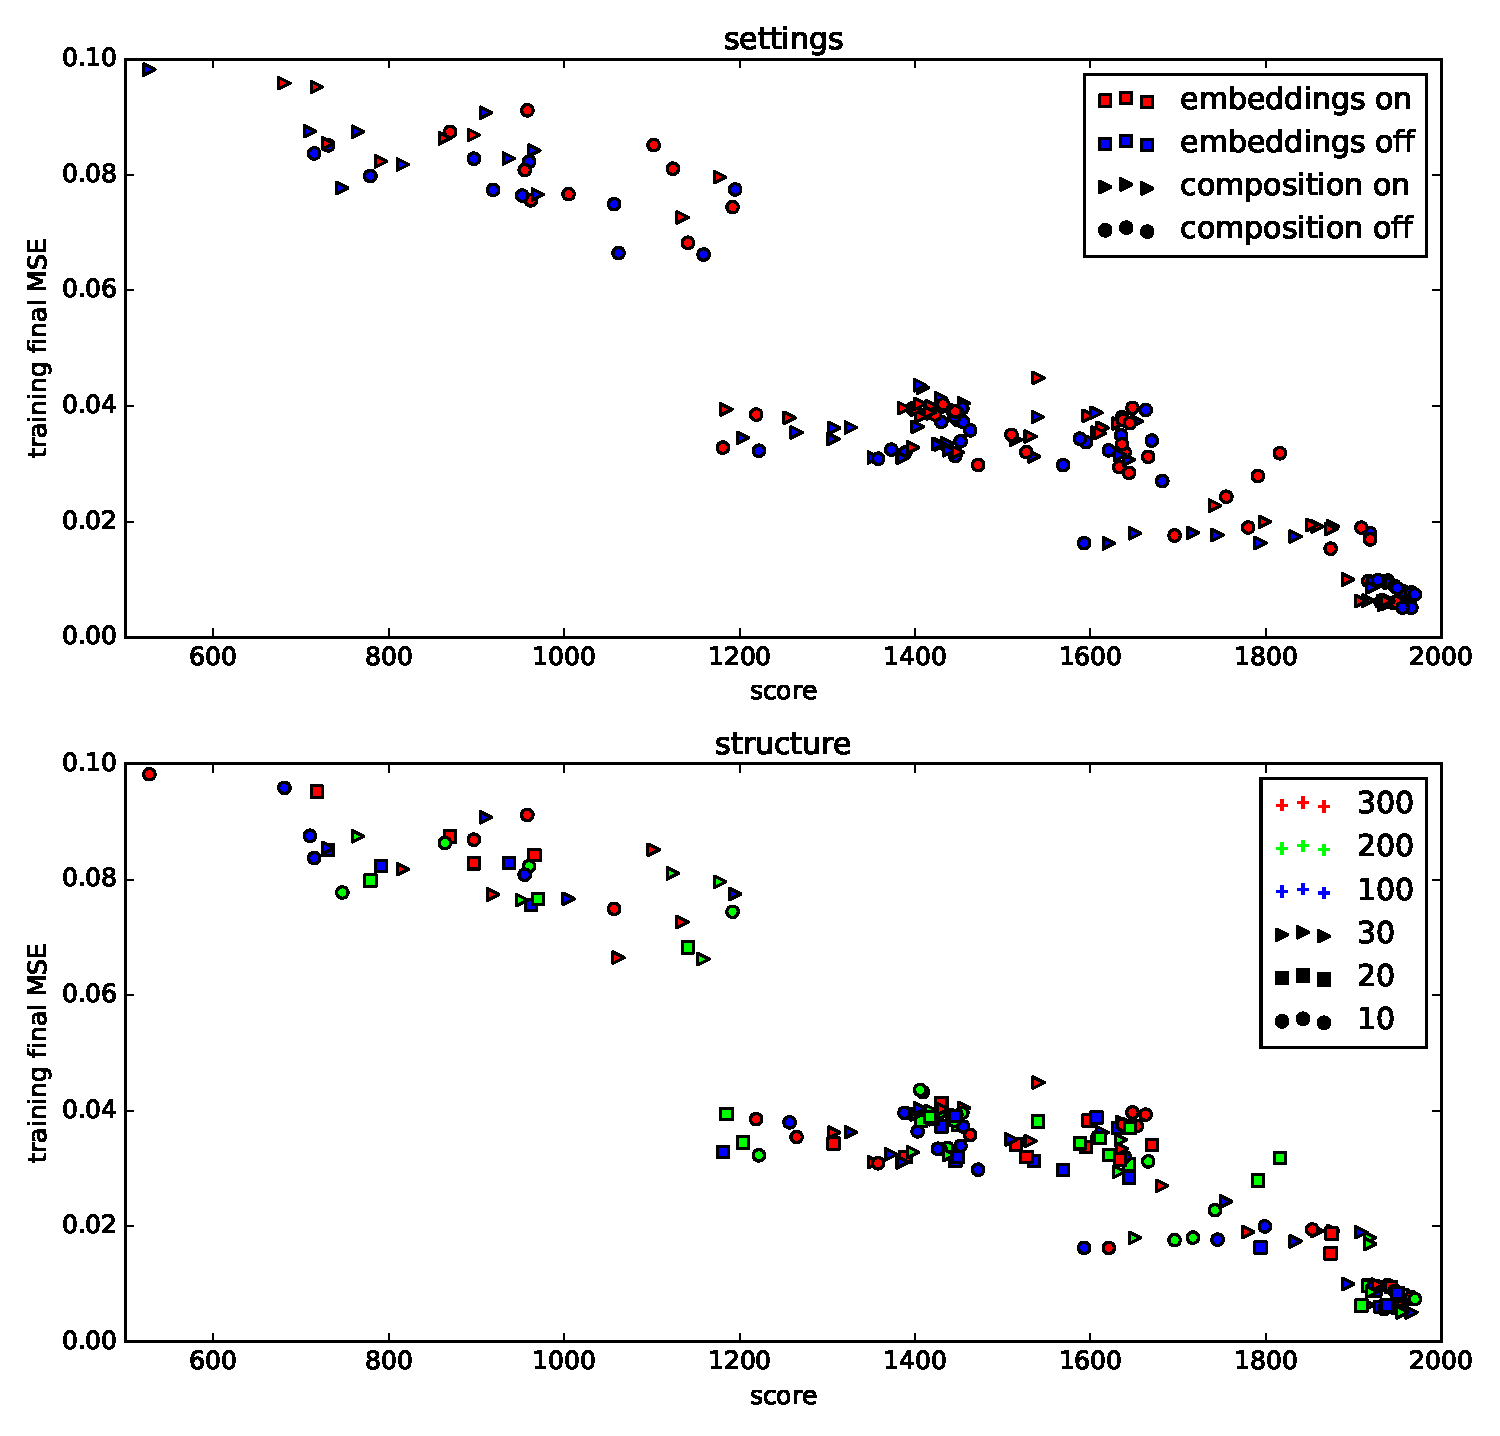
\includegraphics[width=\linewidth]{ext/figure_simples_cmb.pdf}
\caption{The plot shows results on a dataset containing only a simple shapes, without embeddings or conglomeration. Each point represents a single network. The x-axis shows achieved score according to the rules (see \cref{rules}), and the y-axis shows the achieved MSE of the network during training.
The first graph shows by color whether was trained to recognize embeddings, and by shape whether the network was trained to recognize conglomerations.
The second graph shows the structure of the network. The color marks the number of neurons in the first hidden layer and the shape marks the number of neurons in the second hidden layer.}
\label{fig:simples}
\end{figure}

\begin{figure}
\centering
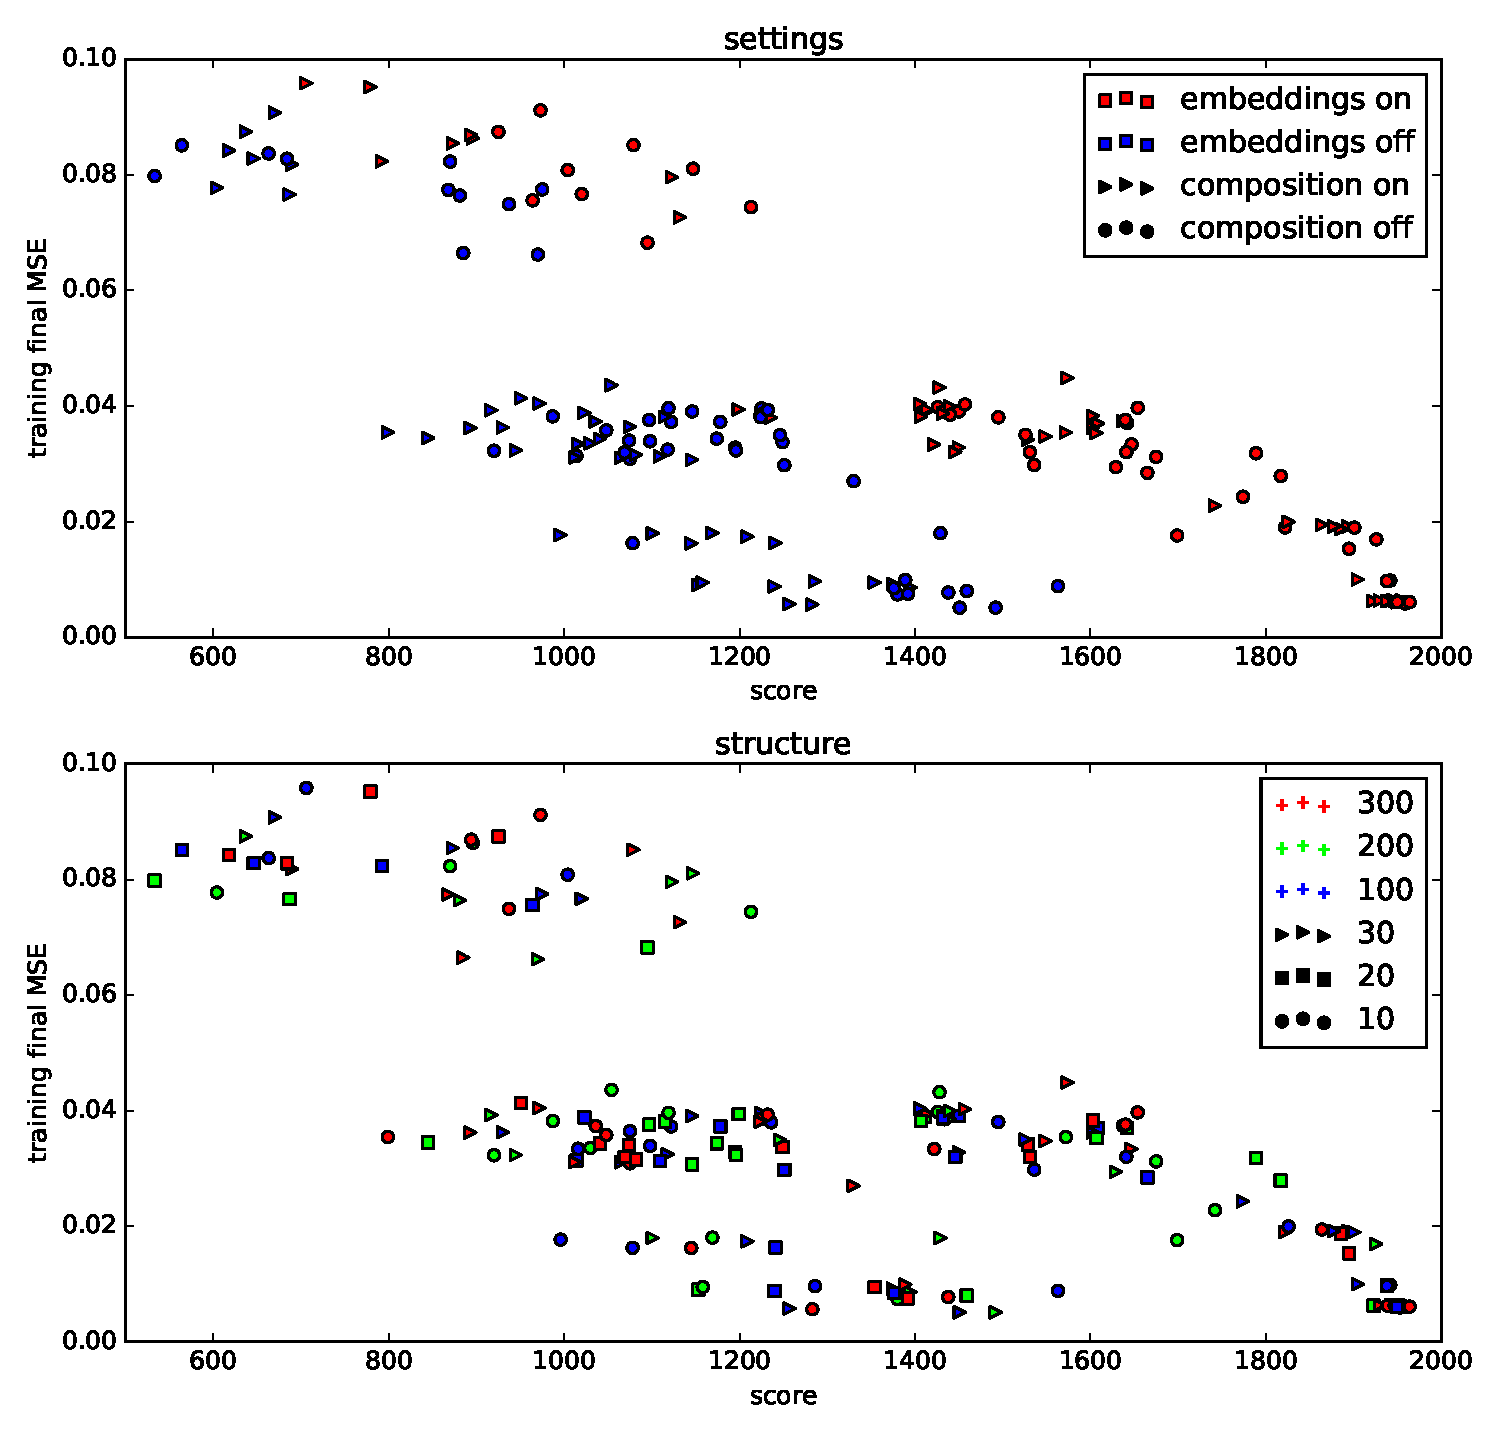
\includegraphics[width=\linewidth]{ext/figure_embed_cmb.pdf}
\caption{The plot shows result on a dataset containing embedded shapes. Each sample  contained shape with an embedded shape. The plot follows the same format as in \cref{fig:simples}.}
\label{fig:embed}
\end{figure}

\begin{figure}
\centering
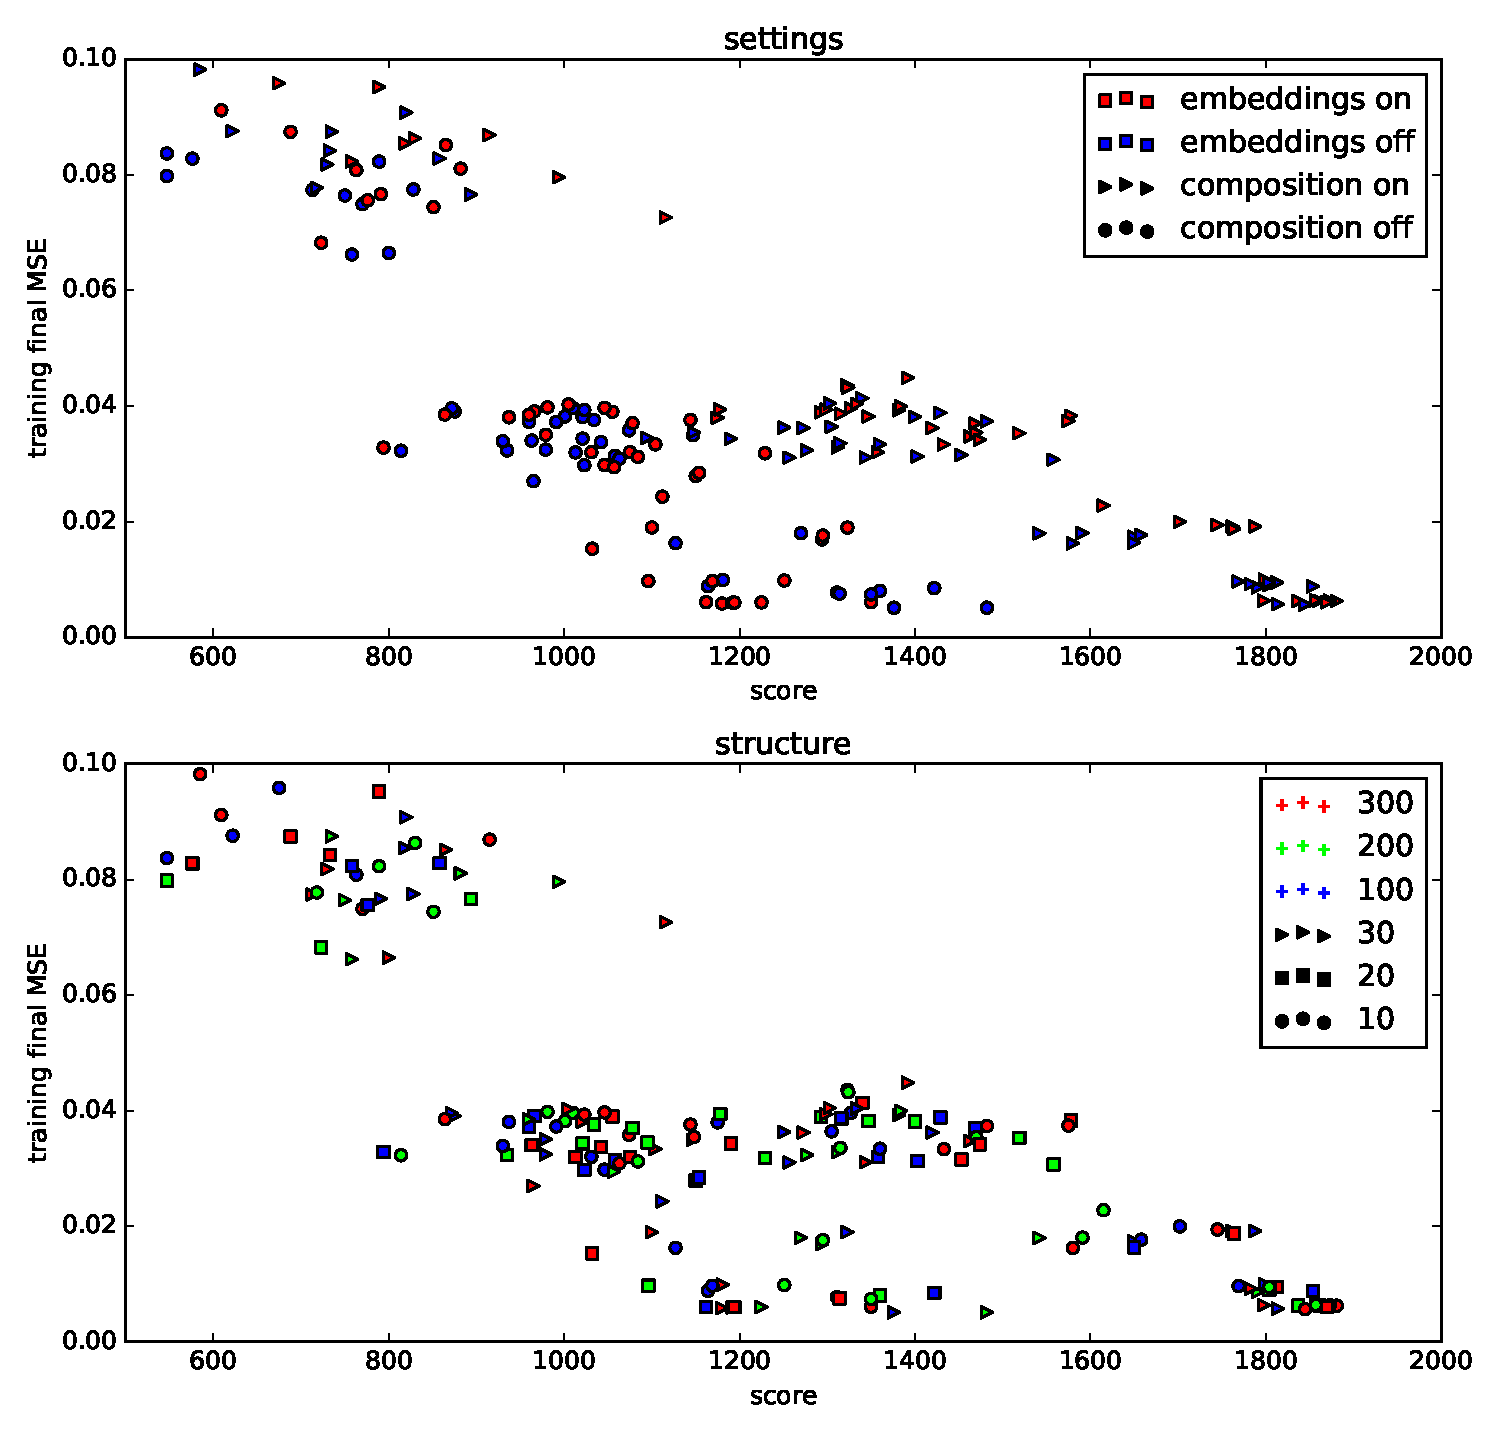
\includegraphics[width=\linewidth]{ext/figure_comp_cmb.pdf}
\caption{The plot shows result on a dataset containing composition of shapes. Each sample  contained shape composed from a number of instances of a pattern shape. The plot follows the same format as in \cref{fig:simples}.}
\label{fig:comp}
\end{figure}

\begin{figure}
\centering
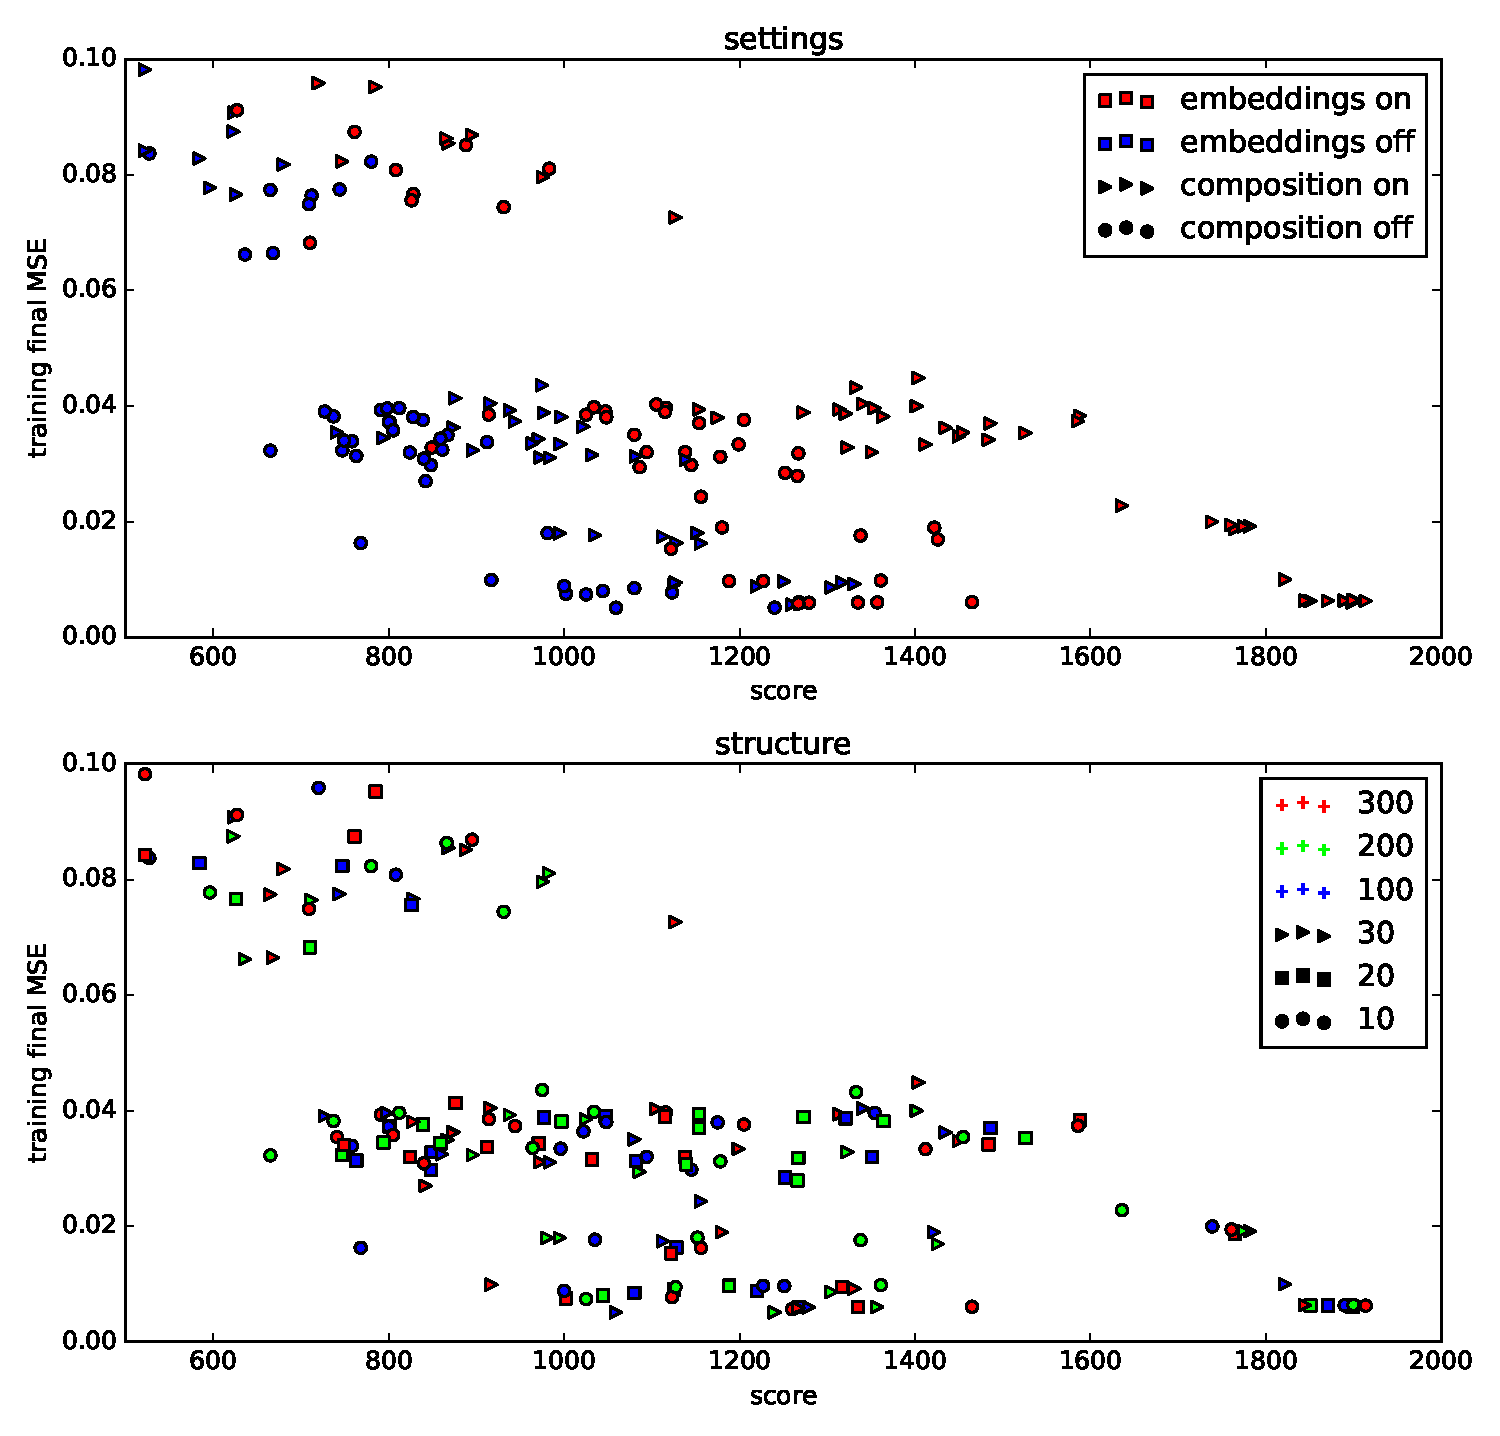
\includegraphics[width=\linewidth]{ext/figure_x_cmb.pdf}
\caption{The plot shows result on a dataset containing combination of embedded and composed shapes. Each sample contained a shape composed from a number of instances of a pattern shape and with an embedded shape. The plot follows the same format as in \cref{fig:simples}.}
\label{fig:cmb}
\end{figure}

There is a visible gap on the y-axis between $0.07$ and $0.04$ in all graphs. This is caused by the a sudden improvement when the network was trained to reach MSE under 0.07. The network usually improved even a little more, finishing the training with a MSE around 0.04 or lower.

Size of the network did not show any visible influence on the network performance. It therefore seems that even the network with the lowest number of neurons is sufficient for this setup, although more neurons might be needed for networks that need to recognize more basic shape descriptors.

It can also be observed from the figures that the tendency to overtrain is not present even with very low MSE. It is therefore preferable to aim for a lower MSE values during training, as that clearly improves the achieved score.

The key result, visible in \cref{fig:simples}, is that training the network to recognize the embeddings and composition effects decreases only slightly the performance on the simple shapes if the network is trained for a low final MSE.

\section{Algorithm parameters optimization}
In this section, we test and evaluate the recognition algorithm performance. In the evaluation, we use the best network trained for both embeddings and composition, since it was observed from the results that the network trained for both cases performs almost as well as networks trained for only one case. We attempt to optimize the algorithm parameters (described in \cref{sec:properties}) for the recognition of the used shape descriptors: square, circle, triangle and water drop. It may be possible that the parameters would have different optimal values for different shape descriptors.

\subsection{Composition recognition}
To measure the precision of recognition of composed shapes we have prepared 100 \texttt{ImageLines} instances of composition examples. Each instance represents a shape composed of instances of another shape. We have also setup the algorithm this way:
\begin{itemize}
\item \texttt{COMPOSED\_SHAPES\_ENABLED = true;} --- Indicates that the algorithm should search for the pattern shape.
\item \texttt{EMBEDDED\_SHAPES\_ENABLED = false;} --- Indicates that the areas of interest defined by \texttt{ShapeDescriptors} are not examined for embeddings.
\item \texttt{ROTATION\_ENABLED = false;} --- Indicates that the shapes should not be analyzed at different rotations.
\end{itemize}
This setting causes the algorithm to search for the pattern shape of the possible composition, but to ignore embeddings locations and to not match different rotations.

We have tested different combinations of settings of these variables:
\begin{enumerate}
\item \texttt{COMPOSITION\_SAMPLES\_COUNT}
\item \texttt{COMPOSITION\_SAMPLES\_LIMIT}
\item \texttt{COMPOSITION\_WINDOW\_SIZE} 
\end{enumerate} Again, see Appendix \cref{sec:properties} for detailed parameter explanation.

For each test instance we have compared the correct pattern shape with the recognized pattern shape.

From the results in \cref{fig:com}, we can see that the success rate grows with the increasing number of samples. The algorithm has more chances to hit the area with the shape, rather than the area between the shapes. Generally the chance to recognize at least one pattern shape is higher.

%obrazky je dobry vkladat okamzite pod mistem kde se o nich mluvi --- latex tak muze podstatne lip odhadnout kde ten obrazek vlastne bude potreba a vysazet to vhodnejc.... tenhle sem presunul trochu zespod.
\begin{figure}
\centering
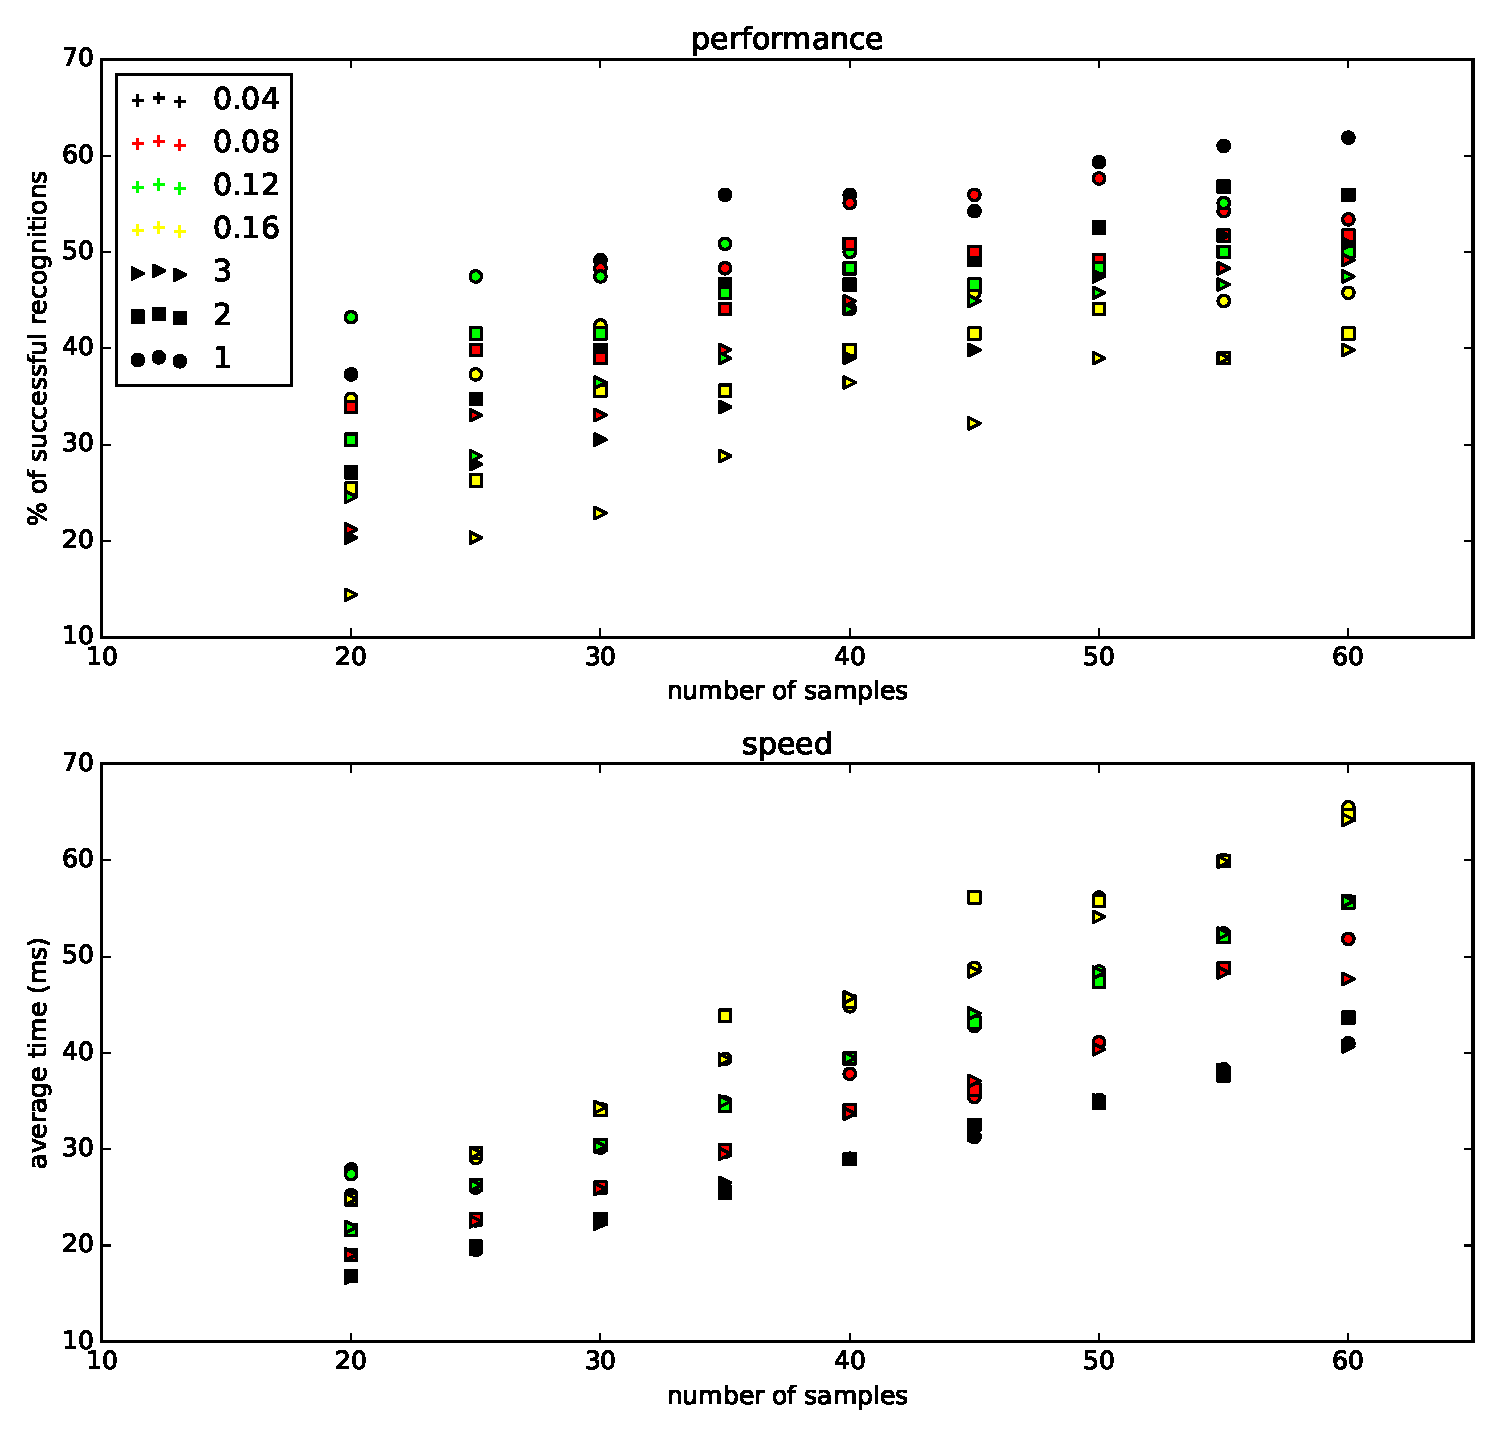
\includegraphics[width=.8\linewidth]{ext/figure_composition_results.pdf}
\caption{The x-axis shows the values of \texttt{COMPOSITION\_SAMPLES\_COUNT}, which is actually a count of samples made around the shape contour. The point color denotes the \texttt{COMPOSITION\_WINDOW\_SIZE}, and the point shape denotes the \texttt{COMPOSITION\_SAMPLES\_LIMIT} according to the legend. Each object of the plot then represents a combination of parameters settings and the performance and speed achieved with the parameters over the test samples. The y-axis of the first plot shows the successful recognitions percentage over the test samples, and in the second plot, the y-axis shows an average computation time per one sample.}
\label{fig:com}
\end{figure}

We can also see that the red and black colors representing the smaller sizes of the sample window perform better with the higher sample count, while being faster at the same time. The performance improvement for the smaller sample window tells us that the network does not recognize the shapes if the surrounding of the area covered by parts of other shapes. The speed difference is caused mainly by rasterization algorithm that needs to process more lines that are found in larger windows.

There is also a sharp drop in success rate when increasing the sample limit to more than one. This means that the network has trouble recognizing even a single pattern shape from the shapes that form the composition. There are two factors that affect the recognition of the pattern shape:
\begin{description}
\item The sampling window follows the ideal path from the shape descriptor, but the real shape is usually more or less deformed, which means that the window will hit only a part of the pattern shape.
\item The pattern shapes can be of various sizes which is hard to approximate by a single size of the sampling window. And if even the window hits the whole pattern shape, there is a very high chance of hitting also the noise from other shape patterns, or from embeddings.
\end{description}
Both factors make the recognition very difficult for the network. The network is rarely able to recognize even a single pattern shape correctly, and after 40 samples, the success rate does not improve much and stays somewhere between 40\% and 60\%.

It is clear that the algorithm becomes gradually slower with the increasing number of samples. The total time will also increase substantially if the rotation is turned on, because each composition sample is tested for all rotations.

\section{Rotation}
Rotation invariance is achieved by redrawing the image at different angles and returning the best match from the rotated samples. We tested the influence of the \texttt{ROTATION\_SAMPLES\_COUNT} variable on the precision and speed of the algorithm. 

In the results \cref{fig:rotation} we can see that the precision of simple data shapes reaches almost 100\% at 15 samples. However, the recognition of the composed shapes is much worse. At 15 samples, it reaches about 70\% success rate and barely improves for the higher sample values. At the same time we know from \cref{fig:cmb} that the network is able to recognize composed shapes quite successfully. 

\begin{figure}
\centering
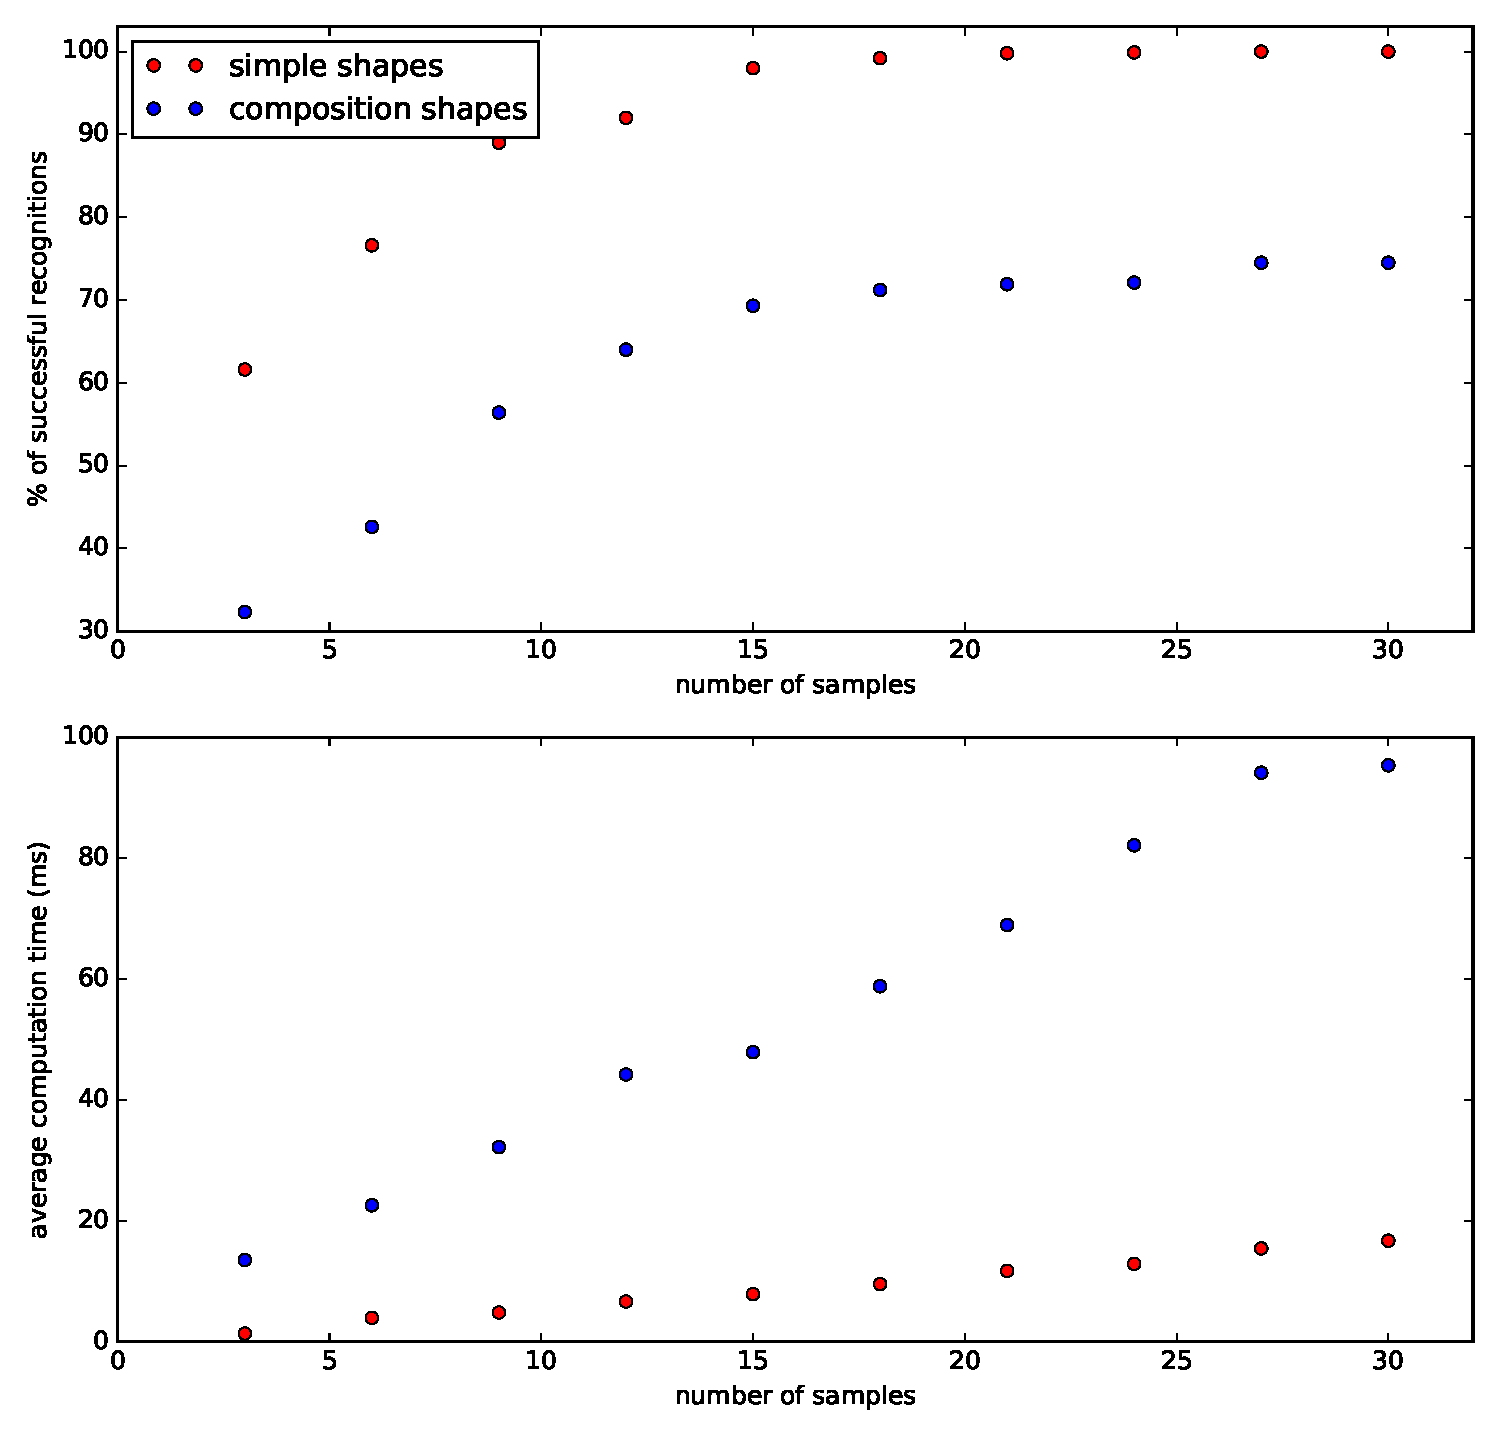
\includegraphics[width=\linewidth]{ext/rotation_cmb.pdf}
\caption{The x-axis shows the values of \texttt{ROTATION\_SAMPLES\_COUNT}. Each dot represents a test run over the test data. The red dots represent results over the test data with simple shapes, and the blue dots represent results over the test data with composed shapes. The y-axis of the first plot shows success recognition rate and in the second plot the y-axis shows an average computation time per one sample.}
\label{fig:rotation}
\end{figure}

From the result data, we conclude that the main cause of the problem are false matches of different shapes. For example, a square composed from circles can, at 45 degrees rotation, closely resemble a circle, and the network assigns the circle a higher match value than the square at the correct rotation.

We can also observe from \cref{fig:rotation}, that the speed of the recognition of composed shapes is much slower and the gap in the performance is increasing with the samples count. This is caused by the fact that composed shapes contain a lot more lines than the simple shapes and each of these lines adds to the transformation time and to the drawing time.

We can deduce that setting \texttt{ROTATION\_SAMPLES\_COUNT} higher than 15 is rather unnecessary.


\section{Embeddings}
The ability of the algorithm to recognize embeddings depends more on the shape descriptor definition rather than on the algorithm settings.

The library user can define the points of interest by their position and size, and these two parameters form a rectangular area where the algorithm will search for embedded shape.

It is then recommended to set the size of this area lower, to avoid fragments of the top shape appearing in this area, which might cause the network to not recognize the embedded shape. If the embeddings are supposed to appear inside composed shapes, the area should be even smaller, otherwise the fragments of the pattern shapes will appear inside.

Embedding matching has a simple influence on the algorithm performance. Every point of interest defined in the \texttt{ShapeDescriptor} is analyzed and if the embedded shape is found, the algorithm runs recursively on the area of the embedded shape.



\chapter*{Conclusion}
The goal of this thesis was to develop a recognition algorithm that recognizes structured combinations, such as conglomerations and embeddings. We have reviewed the literature for pattern recognition and found out that although the topic of recognition of shapes is covered well, approaches to recognition of shape combinations and modifications that this thesis targets are rare. \todo{rict o literature ze je nedostatecna tim puvodnim zpusobem je zasadni strela do vlastnich nohou.} From several reviewed algorithms we have chosen the artificial neural networks as a base for our recognition algorithm. 

We have developed a recognition library that allows users to define their own shapes, train the appropriate neural network and use the library for recognition of structures made from the defined shapes. For the purpose of the neural network learning, we have also developed a shape images generator that attempts to approximate human imprecise drawing.

We have then used the library in a game prototype to demonstrate its functionality. The game supports several defined shapes and their combinations in the form of embeddings and composition, which all systematically map to different spell effects. 

In the last chapter, we have benchmarked the performance of our library and optimized the algorithm parameters for the used shape descriptors. The results suggest that while the success rate of the recognition of composed and embedded shapes is high, the recognition process of the pattern shape of the composition still needs improvements. \todo{pochopil sem to dobre ze je tezky rozpoznavat veci ze kterejch sou poskladany ty vetsi tvary, zejo? (s vysledkama by to sedelo, jen proveruju)}

\section{Future work}
There are several further directions that might be worth exploring:
\begin{itemize}
\item One of the main problems is the noise from the surroundings introduced when extracting the area of embeddings and pattern shapes. Heuristics, like extracting only continuous segments of lines, or neural network with stronger generalization power, might be used to improve the recognition.

\item Speed \todo{performance} of the algorithm might be an issue in more demanding game environments. While \todo{Apart from the fact that?} the analysis of several images can be performed in parallel, the algorithm can be even further parallelized. The large number of relatively simple repeated computations is especially well suited for being run on GPU.

\item Developing a playable, gamer-targeting game that uses the library would be a great final step of the development. The provided game prototype is arguably not very well suited for the gamers (which will find it boring after several spells), nor for the library: The game currently forces the players to draw shape during combat and while moving the character, resulting time stress discourages the player from trying out more complex shapes.

For example, a strategy game might be a better candidate. Instead of building the base with player's units, players could create them by drawing the correct shape. The advanced shape structures would then create buildings with stronger units.

Using an input controller that is more suitable for drawing than a mouse might also greatly enhance the player experience.
\end{itemize}


%%% Bibliography
%%% Bibliography (literature used as a source)
%%%
%%% We employ bibTeX to construct the bibliography. It processes
%%% citations in the text (e.g., the \cite{...} macro) and looks up
%%% relevant entries in the bibliography.bib file.
%%%
%%% The \bibliographystyle command selects, which style will be used
%%% for references from the text. The argument in curly brackets is
%%% the name of the corresponding style file (*.bst). Both styles
%%% mentioned in this template are included in LaTeX distributions.

% \bibliographystyle{plainnat}    %% Author (year)
% \bibliographystyle{unsrt}     %% [number]
\bibliographystyle{alpha}

\renewcommand{\bibname}{Bibliography}

%%% Generate the bibliography. Beware that if you cited no works,
%%% the empty list will be omitted completely.

\bibliography{bibliography}

%%% If case you prefer to write the bibliography manually (without bibTeX),
%%% you can use the following. Please follow the ISO 690 standard and
%%% citation conventions of your field of research.

% \begin{thebibliography}{99}
%
% \bibitem{lamport94}
%   {\sc Lamport,} Leslie.
%   \emph{\LaTeX: A Document Preparation System}.
%   2nd edition.
%   Massachusetts: Addison Wesley, 1994.
%   ISBN 0-201-52983-1.
%
% \end{thebibliography}

\chapter{User guide}
\todo{Tohle je tradicne Appendix --- pro vlastni text prace to neni moc podstatny, krome toho ze tam chces nekam velice jednoduse (idealne v obrazku) popsat to API a rict proc je skvely, a pak se jen odkazes na appendix kde to vysvetlujes.}
\section{Recognition system}
\todo{ schema and interface overview - files IMageAanlyzer and training}

\subsection{Creation of shape descriptor}
For both the training and for the recognition shape descriptors are required. The shape descriptors have several rules, that need to be followed by the user in their implementation. The intended purpose of the descriptor is to describe a single 2D shape in a $[0,1]^2$ rectangular area. The descriptor is expected to return the exactly same shape every time and all of its methods should return the same values when called with the same parameters. 

It is also required, that all of the shape descriptor methods are thread safe. It is then recommended to design the shape descriptor as a class with a constant inner state. Not following these rules may result in an unexpected and dysfunctional behavior of the system. 

The user can create a shape descriptor by including the \texttt{ImageAnalyzer.h} header file and inheriting from the class \texttt{ShapeDescriptor}. This class contains several abstract methods, that should be implemented:
\begin{description}
\item[\texttt{GetName()}] Returns the name of the shape a string. This is only for debugging purposes and it does not have to be unique or even constant. However, it is recommended to return a constant unique name among the descriptors.

\item[\texttt{GetPoint(\texttt{float} t)}] Function overload with one parameter \texttt{t} should return a point on the contour of the shape, based on the \texttt{t} parameter. It is recommended to normalize the parameter into $[0,1]$ range by \texttt{NormalizeParam} function.

\item[\texttt{GetPoint(float last\_t, float t, float \& point)}] Function overload with three parameters, that allows the descriptor to describe noncontinuous curves. The \emph{point} parameter passed by a reference should be filled with the same value as from \texttt{GetPoint(t)} as it describes the point of the curve. Then the function should return true if the curve is continuous on the interval $[last\_t, t]$, otherwise false.

\item[\texttt{GetPointsOfInterest()}] Function, that describes places, where an embedded shape may appear. It returns a vector of \texttt{float3} type, where the first two numbers denote the top left corner of the square area, and the third number is the size of the square. It is important for the correct functionality that the points of interest do not overlap with the shape curve, and that they are substantially smaller than the parent shape.
\end{description}

Examples of shapes descriptors can be found in the \texttt{ExampleShapeDescriptors.h} file. Be careful to return the points only in the normalized range $[0,1]^2$.

\subsection{Algorithm properties}
There are several variables then can be set up and influence the functionality of the software. They can be found in the \texttt{ImageAnalyzer} namespace. Some of them are used both in the training and in the recognition. It is necessary then for the user to be consistent and use the same settings for the recognition as they used for the training.

\begin{description}
\item[\texttt{DEBUG\_IMAGE\_SAVE}] Boolean variable with default value false. Only for debugging purposes. If true, the images created during the recognition are saved as BMP files onto the hard disk into folder \texttt{debug/}, but only in the initial rotation of the image.

\item[\texttt{COMPOSED\_SHAPES\_ENABLED}] Boolean variable with default value true. If false, recognition algorithm recognizes the whole shape but does not search for the pattern shape that might compose it. During training, the generating algorithm does not produce compositions of the shape, so the network is not trained to recognize the composed shapes.

\item[\texttt{COMPOSITION\_SAMPLES\_COUNT}] Integer variable describing the amount of samples taken when searching for the pattern shapes. This variable has no effect when composed shapes are disabled. Otherwise, the interval $[0,1]$ is sampled uniformly and each sample is passed into the \texttt{GetPoint} method of the descriptor. The returned point is then expanded into the sampling window and checked for pattern shape.

\item[\texttt{COMPOSITION\_WINDOW\_SIZE}] Float variable that describes the size of the sampling window used during pattern shape matching. The actual window is a square with a side size of 2*\texttt{COMPOSITION\_WINDOW\_SIZE}. This variable has no effect when composed shapes are disabled.

\item[\texttt{COMPOSITION\_SAMPLES\_LIMIT}] Integer variable describing the number of minimum pattern shape matches. If the count of the pattern shape matches is lower, the pattern shape is not recognized. This variable has no effect when composed shapes are disabled.

\item[\texttt{EMBEDDED\_SHAPES\_ENABLED}] Boolean variable with default value true. If false, recognition algorithm ignores the \texttt{GetPointsOfInterest} method of the shape descriptor, where embedded shapes might be, and recognizes only the top level shape and its composing shape. During training, the generating algorithm will not generate embedded shapes, and the network will not be trained to filter out these locations, where the embeddings could appear.

\item[\texttt{ROTATIONS\_ENABLED}] Boolean variable with default value true. If false, recognition algorithm will not test different shape rotations for the best match, but will use the initial rotation. This variable does not have an impact on training since rotation recognition is not a direct task of the neural network.

\item[\texttt{ROTATION\_SAMPLES\_COUNT}] The amount of samples created when matching rotated shape. It directly determines the rotation step angle size, which is in degrees 360/\texttt{ROTATION\_SAMPLES\_COUNT}. This variable has no effect when rotations are disabled.

\item[\texttt{DEBUG\_OUPUT}] Integer variable with default value 1. Controls the amount of debug info of the recognition system. If set to 0 or lower, no debug output is produced. If set to value 1, it prints recognized shape with its matching rotation and its composing shape to the standard output, for the top level shape and each embedded shape. If set to 2 or higher, produces the same output as with value 1, but also all network outputs from the analysis are printed for all the rotations.

\item[\texttt{IMAGE\_SIDE\_SIZE}] Integer variable, controls the size of the images that are created anytime during algorithm. Every time there is an instance of \texttt{ImageLines} class that should be analyzed by the network, the lines are drawn into the square pixel map of a size set by this variable and then serialized as an input to the network. The network input layer size has to be the second power of this value. The default value is 32, which means that the neural network has an input layer of size 1024 neurons, and the images produced in the algorithm are pixel maps of $32*32$ pixels.

\end{description}

\subsection{Training phase}
Training the neural network consists of several steps. The first step is to set up the variables controlling the behavior of the recognition and training algorithms. By including the \texttt{Training.h} file, the user can access the \texttt{ImageAnalyzer} namespace for setting up the variables, and the \texttt{Training} namespace for the training functions. 
After setting the variables, it is necessary to register the desired shape descriptors through function the \texttt{Training::RegisterShapeDescriptor}. This function takes a unique pointer to the shape descriptor as its parameter, and returns an instance of the \texttt{ShapeIndex} class. This class is only a wrapper over integers but it works as an identifier of the shape in the algorithm and the calls to the \texttt{ImageAnalyzer::Analyze} will return the \texttt{ShapeIndex} for each recognized shape. 
The next step is to call the \texttt{Training::Train} function. This function has several parameters:
\begin{description}
\item \texttt{std::string name} Describes the name of the neural network. When the network is created and trained, it is saved under the current working directory into the file with the name \texttt{name} with the extension \texttt{.net}.
\item \texttt{vector<unsigned int> networkStructure} This parameter describes the layers of the network. Each number represents number of neurons in a single layer. The first number describes the size of the input layer, while the last number describes the size of the output layer. The user can set any number of layers higher than two, and arbitrary sizes of layers, apart from the first and last layer.  The first layer has to be equal to the second power of \texttt{IMAGE\_SIDE\_SIZE}, and the last layer size has to be equal to the number of registered shape descriptors.
\item \texttt{boolean generateData = true} Parameter that controls whether the training algorithm should generate the training data. The algorithm looks for training data in the current working directory in the file \texttt{training.data} and for test data in file \texttt{test.data}. If the parameter is true, the algorithm will generate these two files, possibly overwriting them. If the parameter is false, the algorithm uses the files found, or ends with error, of the files are not found.
\item \texttt{float targetMSE = 0.01} The MSE that the network should achieve on the \texttt{test.data}. The training stops if the network achieves MSE lower than this value, or if the network does not improve anymore. 
\item \texttt{int dataSize = 300 000} The parameter describing the number of generated training samples in the \texttt{training.data}. The size of the generated test data is one third of this value. if the parameter \texttt{generateData} is false, then this parameter is ignored. 
\end{description}
after the training process finishes, the network is ready to be used in the recognition algorithm.

\subsection{Recognition phase}
When the neural network is ready, the user can set up the recognition system and use it in a game. The recognition system is used through interface located in the \texttt{ImageAnalyzer} namespace in \texttt{ImageAnalyzer.h} file. The namespace contains definition of the algorithm properties, as well as definition for classes that the user is supposed to use, namely the \texttt{ShapeDescriptor} class, the \texttt{ImageLines} class and the \texttt{ShapeIndex} class.

First, it is necessary to load the neural network into the algorithm, using \texttt{ImageAnalyzer::LoadNetwork} function, which takes string describing the path to the network as an argument. Then, the user has to register the same descriptors used for the training of the loaded network again, but this time using the \texttt{ImageAnalyzer::RegisterShapeDescriptor}, which takes the corresponding \texttt{ShapeIndex} instance together with the descriptor.

Alternatively, the \texttt{ShapeIndex} instance can be created from the order number of the corresponding shape descriptor when registered for the training. It is also necessary to set up the algorithm properties the same way they have been set up during network training. When these steps are done, the user can repeatedly call the \texttt{ImageAnalyzer::Analyze} function to determine the shape hierarchy in the provided \texttt{ImageLines} instance. The \texttt{Analyze} function is thread safe, so many calls can be done at the same time. However, the set up has to be done synchronously and only once, before the first call of \texttt{Analyze} function. 

\section{Game}
TODO

%\listofalgorithms

%%% Figures used in the thesis (consider if this is needed)
%\listoffigures

%%% Tables used in the thesis (consider if this is needed)
%%% In mathematical theses, it could be better to move the list of tables to the beginning of the thesis.
%\listoftables

%%% Abbreviations used in the thesis, if any, including their explanation
%%% In mathematical theses, it could be better to move the list of abbreviations to the beginning of the thesis.
%\chapwithtoc{List of Abbreviations}
%\renewcommand{\nomname}{List of Abbreviations}
%\printnomenclature

%%% Attachments to the bachelor thesis, if any. Each attachment must be
%%% referred to at least once from the text of the thesis. Attachments
%%% are numbered.
%%%
%%% The printed version should preferably contain attachments, which can be
%%% read (additional tables and charts, supplementary text, examples of
%%% program output, etc.). The electronic version is more suited for attachments
%%% which will likely be used in an electronic form rather than read (program
%%% source code, data files, interactive charts, etc.). Electronic attachments
%%% should be uploaded to SIS and optionally also included in the thesis on a~CD/DVD.
\chapwithtoc{Attachments}

\section*{Attachment A --- the Enclosed CD}

On the CD attached to this thesis we enclose the source codes of the implemented software together with the source codes of its dependencies \citet{urho} engine and \citet{fann}.

The electronic version of this thesis is also enclosed.

\openright
\end{document}

